\documentclass{llncs}
\usepackage{amssymb}
\usepackage{graphicx}
\usepackage[ruled,linesnumbered,boxed]{algorithm2e}
\usepackage{graphicx}
\usepackage{amsmath}
%\usepackage{mathtools}
%\usepackage{color}
\usepackage{tabularx}
\usepackage[colorlinks, linkcolor=blue, anchorcolor=blue, citecolor=green]{hyperref}
%\usepackage{booktabs}
\usepackage[table]{xcolor}
%\uespackage{colortbl}
\usepackage[tight,footnotesize]{subfigure}
\usepackage{fancyhdr}
\usepackage{lastpage}
\usepackage{layout}
%\usepackage{ctex}

%\footskip = 10pt
\pagestyle{fancy}
\chead{Group Project}
\lhead{CS214-Algorithm@SJTU}
\rhead{Instructor: Xiaofeng Gao}
\rfoot{}
\cfoot{Page \thepage \ of \pageref{LastPage}}
\addtolength{\headheight}{0.5\baselineskip}
\addtolength{\headwidth}{0\marginparsep}
\addtolength{\headwidth}{0\marginparwidth}



\title{DAG Job Scheduling Across Geo-Distributed Datacenters}
\subtitle{A Multifunctional, Effective Scheduler Achieving Max-Min Fairness \vspace{-3mm}}

\author{Li Zenan (519021911033, Emiyali@sjtu.edu.cn), Fang Tiancheng (519021910173, fangtiancheng@sjtu.edu.cn), Dou Yiming (519021910366, douyiming@sjtu.edu.cn)}
\institute{Department of Computer Science, \\ Shanghai Jiao Tong University, Shanghai, China}

\begin{document}
\bibliographystyle{splncs}

%\linespread{0.85}

%==============================================================================
\maketitle
\begin{abstract}\vspace{-5mm}
Job scheduling across distributed data-centers is an important problem of computer science is a \textbf{NP-complete} problem, which is proven in this paper, so there has not been any efficient method to solve the problem in polynomial time. Therefore, we focus on the optimization algorithms such as \textbf{heuristic algorithm} and \textbf{linear programming} to approximately get the optimal solution in finite time. Our work includes the problem formalization, data preprocessing, proof of the hardness, algorithm design and the test on various data-sets.

In terms of the problem formalization, we formulate models and define the \textbf{max-min fairness} and thus determine our goal. Then, we give assumptions of the model and decide to design $3$ models based on the different extents of the strictness.

As for data preprocessing, we begin with separating the tasks into stages based on \textbf{topological sort}. Furthermore, we update the bandwidth between each data-center by transferring data through middle transfer stations.

When it comes to the proof of hardness, we reduce our problem from Job Shop Scheduling Problem (JSP), which is proven to be NP-hard.

With regard to the algorithm design, we gradually make the constraints more and more strict and design $3$ models based on different strictness. \textbf{Genetic Algorithm} and \textbf{SJF} algorithm is respectively used for the loose and medium strictness. For the strict situation, we use the \textbf{linear programming} model to strictly find the optimal scheduling method.

Eventually, we test the performance and efficiency on the toy-data and conduct further experiments on larger data-sets randomly generated by us. Furthermore, we compare the different algorithms with each other and the baseline, showing the pros and cons of each model.

\textbf{Keywords:} Genetic Algorithm, SJF, Linear Programming, max-min fairness, multi-job scheduling
\end{abstract}
\section{Introduction}

    Scheduling computational tasks, as commonly represented by directed acyclic graphs (DAGs), is an important problem in many areas of computer science ranging from programming language (e.g., compilation), operating systems (e.g., parallel processing), data engineering (e.g., distributed batch/streaming computation topology), to machine learning (e.g., training graphs). 
    
    Fig. \ref{fig:intro} shows an example of scheduling multiple jobs across geo-distributed data centers.
    \begin{figure}
        \centering
        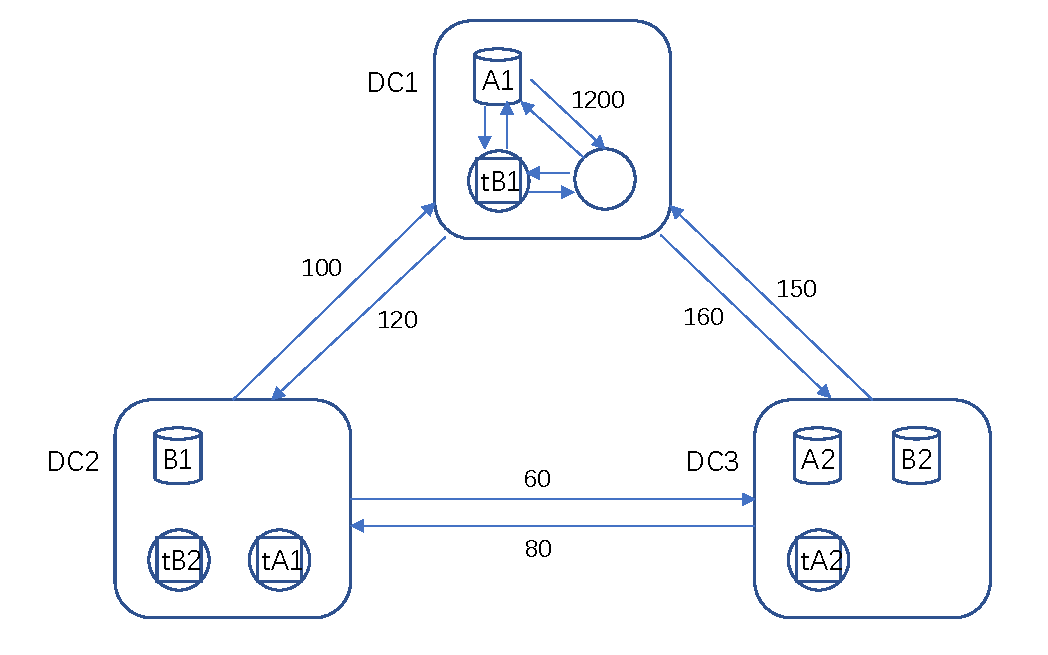
\includegraphics[width=10cm]{Figures/Intro.pdf}
        \caption{An example of scheduling multiple jobs across
            geo-distributed data centers}
        \label{fig:intro}
    \end{figure}
    
    The DAG scheduling problem is a combination of two well-known NP-hard problems: the Job Shop Scheduling Problem (JSP) \cite{ref_6} and the Bin Packing Problem (BPP) \cite{ref_7,ref_8}. On the one hand, if we let the network bandwidth be infinite and the DAG degenerates into a line segment, the DAG scheduling problem then degenerates into JSP. Furthermore, if we fix the network transmission cost and computation cost, then the DAG scheduling problem will degenerate into BPP. Anyway, there is no effective algorithm to find the optimal solution of this problem up to now. All the proposed algorithms are either greedy algorithms, or based on machine learning \cite{ref_9} or heuristic search.

    In this paper, we describe the DAG scheduling problem in mathematical language. Then we relax the assumption step by step, presenting three methods to solve the problem.
    
    \textbf{Firstly}, we strictly assume that all data centers have unlimited slots. Every task arriving at the data center can be processed immediately. In addition, we also assume that the bandwidth does not contribute to the transmission of tasks between data centers. In other words, when a fixed size task is transferred from one data center to another, the time is fixed regardless of other tasks. In this condition, we propose a task coding method and its {\bf Genetic Algorithm}. Our method can get a solution (17.65s) which can not be further optimized at a very fast speed(about 0.8s) for toy-data.

    \textbf{Secondly}, we remove the hypothesis of unlimited slots. If a ready task arrives at a data center, it may still be rejected if all the slots in the current data center are occupied. In this case, we propose a task simulation system, which uses short task first strategy (SJF) and stochastic optimization method to get the optimal solution. This method can also get the optimal solution in a little longer time (about 2s) than the first method.
    
    \textbf{Thirdly}, on the basis of paper \cite{ref_11}, we propose a linear programming algorithm which is more rigorous than the first two heuristic algorithms. This method makes full use of convex optimization, linear programming and other mathematical means, which not only defends the max-min fairness between tasks, but also optimizes the longest job complete time.

    Next, we write a large-scale data generator to check the robustness of our algorithms. Finally, we analyze the complexity, advantages and disadvantages of our algorithms.
    
\section{Hardness of DAG Scheduling Problem}

We claim that the decision version of DAG Scheduling Problem is a NP-complete problem. Next is the proof, and our proof idea is:
\begin{enumerate}
    \item Show that Job Shop Scheduling Problem is a NP-hard problem.
    \item Prove that the decision version of DAG Scheduling Problem is in NP.
    \item Prove that Job Shop Scheduling Problem $\le_p$ DAG Scheduling Problem.
\end{enumerate}

\textbf{Firstly}, let's start with Job Shop Scheduling Problem(JSP). The standard version of the problem is where you have $n$ jobs $J_1, J_2, \cdots, J_n$. Within each job there is a set of operations $O_1, O_2, \cdots, O_n$ which need to be processed in a specific order (known as Precedence constraints). Each operation has a specific machine that it needs to be processed on and only one operation in a job can be processed at a given time. A common relaxation is the flexible job shop where each operation can be processed on any machine of a given set (the machines in the set are identical).

We claim that JSP problem is a NP-hard problem. Since the Traveling Salesman Problem(TSP)\cite{ref_10} is NP-hard, the job-shop problem with sequence-dependent setup is clearly also NP-hard since the TSP is a special case of the JSP with a single job, imagine that the cities are the machines and the salesman is the job.

\textbf{Secondly}, we need to discuss the decision version of DAG Scheduling problem that whether we could verify a solution, whose makespan is no more than a given number $k$. The earliest thing we need to do is to check the correctness of the solution. We not only need to check whether the tasks can be transmitted under the given bandwidth, but also check whether the prerequisite tasks are completed at the beginning. Of course, these tests can be completed in linear time, because a single test only needs to do some subtraction and judgment. That is to say, the decision version of DAG Scheduling Problem is in NP.

\textbf{Thirdly}, we claim that Job Shop Scheduling Problem can be polynomially reduced to DAG Scheduling Problem. Imagine that all the bandwidth be infinite and the DAG degenerate to a line, and the data required by each task is distributed in a fixed DC, and the size is high-order infinity than bandwidth. Under this assumption, we get the Job Shop Scheduling Problem: Tasks need to be completed on a fixed machine, and tasks need to be executed in strict order.

All in all, the decision version of DAG Scheduling Problem is a NP-complete problem.

\section{Problem Formalization}
\subsection{Symbol Table}
The symbols used in this paper and their definitions are listed as following:
\begin{table}[htbp]
    \centering
    \caption{Symbol Definition}
    \begin{tabular}{|c|c|}
    \hline
        {\bf Symbol} & {\bf Description} \\ \hline
        $\mathcal{K}=\{1,2,...,K\}$ & A set of data parallel jobs \\ \hline
        $\mathcal{D}=\{1,2,...,J\}$ & A set of geo-distributed datacenters \\ \hline
        $\mathcal{T}_k=\{1,2,...,n_k\}$ & Each job $k \in \mathcal{K}$ has a set of parallel tasks \\ \hline
        $a_j$ & The capacity of available computing slots in datacenter $j \in \mathcal{D}$ \\ \hline
        $c_{i,j}^k$ & The time to fetch data for task $i \in \mathcal{T}_k$ if it's assigned to datacenter $j$ \\ \hline
        $e_{i}^k$ & The execution time of task $i \in \mathcal{T}_k$ \\ \hline
        $x_{i,j}^k$ & The assignment of task $i \in \mathcal{T}_k$, it should be 1 when $i$ is assigned to datacenter $j$, otherwise 0 \\ \hline
        $S_i^k$ & The set of datacenters where the input data of task $i \in \mathcal{T}_k$ are stored \\ \hline
        $d_i^{k,s}$ & The amount of input data for task $i \in \mathcal{T}_k$ from $s \in S_i^k$ \\ \hline
        $b_{s,j}$ & The bandwidth of the link from datacenter $s$ to datacenter $j$ \\ \hline
        $\tau_k$ & The lowest task finish time of job $k$ \\ \hline
        $\langle v \rangle_k$ & The $k$th largest element of $\mathbf{v} \in \mathbb{Z}^k$ \\ \hline
        $M$ & $M=J\sum_{k=1}^Kn_k$ where $J$ is the total number of datacenters and $n_k$ is the number of tasks in job $k$ \\ \hline
        $\lambda_{i,j}^{k,s} \in \mathbb{R}^+, s\in\{0,1\}$ & Newly introduced variables when using $\lambda$-representation technique \\
    \hline
    \end{tabular}
    \label{tab:Symbols}
\end{table}

\subsection{Max-Min Fairness}
In this section, we give out the formal definition of {\bf Max-Min Fairness} and transform it into a simpler form to be implemented.

\begin{definition} {\rm \cite{ref_12}}
\label{def:maxmin}
We say that an allocation vector $\mathbf{x}^0$ is said to be max-min fair in $X$ if $\mathbf{x}^0 \in X$ and $\mathbf{x}^0$ fulfills the following property:

For any allocation vector $\mathbf{x} \in X$ and for any connection $d$ such that $x_d > x_d^0$ there exists a connection $d'$ such that $x_{d'} \leq x_{d'}^0 \leq x_d^0$.
\end{definition}

To have a more directive intuition of this , we give out following auxiliary definitions:
\begin{definition} {\rm \cite{ref_11}}
Let $\langle \mathbf{v} \rangle_k$ denote the $k$th ($1 \leq k \leq K$) largest element of $\mathbf{v} \in \mathbb{Z}^K$, implying $\langle \mathbf{v} \rangle_1 \geq \langle \mathbf{v} \rangle_2 \geq ... \geq \langle \mathbf{v} \rangle_K$. Intuitively, $\langle \mathbf{v} \rangle = (\langle \mathbf{v} \rangle_1, \langle \mathbf{v} \rangle_2, ... , \langle \mathbf{v} \rangle_K)$ represents the non-increasingly sorted version of $\mathbf{v}$.
\end{definition}

\begin{definition} {\rm \cite{ref_11}}
For any $\mathbf{\alpha} \in \mathbb{Z}^K$ and $\mathbf{\beta} \in \mathbb{Z}^K$, if $\langle \mathbf{\alpha} \rangle_1 < \langle \mathbf{\beta} \rangle_1$ or $\exists k \in \{2,3,...,K\}$ such that $\langle \mathbf{\alpha} \rangle_k < \langle \mathbf{\beta} \rangle_k$ and $\langle \mathbf{\alpha} \rangle_i < \langle \mathbf{\beta} \rangle_i, \forall i \in \{1,...,k-1\}$, then $\mathbf{\alpha}$ is lexicographically smaller than $\mathbf{\beta}$, represented as $\mathbf{\alpha} \prec \mathbf{\beta}$. Similarly, if $\langle \mathbf{\alpha} \rangle_k = \langle \mathbf{\beta} \rangle_k, \forall k \in \{1,2,...K\}$ or $\mathbf{\alpha} \prec \mathbf{\beta}$, then $\mathbf{\alpha}$ is lexicographically no greater than $\mathbf{\beta}$, represented as $\mathbf{\alpha} \preceq \mathbf{\beta}$.
\end{definition}

In a word, Definition~\ref{def:maxmin} just tells that a vector $\mathbf{x}^0$ is said to be max-min fair if and only if it is the lexicographically smallest vector in $X$.

\subsection{Assumption}
\begin{itemize}
    \item We assume the nodes in the graph are fully connected, that is, we don't need to divide the bandwidth from one datacenter to another.
    \item We always assume that the total slots number is bigger than the total task number, that is, the linear equations will always have a solution.
    \item We don't consider prefetch in this model.
    \item We assume tasks in different jobs could run in parallel while tasks in different states should execute in order.
\end{itemize}

\subsection{Model And Formulation}
Considering a set of data parallel jobs $\mathcal{K} = \{1,2,...,K\}$ submitted to the scheduler for task assignment. For convenience, we first discuss the case that all the tasks could run in parallel, without the constraint of states.

Each job $k \in \mathcal{K}$ will have a set of parallel tasks $\mathcal{T}_k = \{1,2,...,n_k\}$, and for each task $i \in \mathcal{T}_k$, the time it takes to complete consists of both the network transfer time, denoted by $c_{i,j}^k$, to fetch the input data if the task is assigned to datacenter $j$, and the execution time represented by $e_{i,j}^k$. 

For $c_{i,j}^k$, it's determined by both the amount of data to be read, and the bandwidth on the link the data transfers.  Let $S_i^k$ denote the set of datacenters where the input data of task $i$ from job $k$ are stored, the task needs to read the input data from each of its source datacenters $s \in S_i^k$, the amount of which is $d_i^{k,s}$. Let $b_{s,j}$ denote the bandwidth of the link from datacenter $s$ to datacenter $j$, $c_{i,j}^k$ should be the maximum of all the transfer time from the task's source datacenters, that is:
\begin{equation*}
    c_{i,j}^k = \mbox{max}_{s \in S_i^k} d_i^{k,s}/b_{s,j}
\end{equation*}

We use a binary variable $x_{i,j}^k$ to represent the assignment of a task, indicating whether the $i$th task of job $k$ is assigned to datacenter $j$. A job $k$ completes when its slowest task finishes, thus the job completion time of $k$, represented by $\tau_k$, is determined by the maximum completion time among all of its tasks, expressed as follows:
\begin{equation*}
    \tau_k = max_{i \in \mathcal{T}_k, j \in \mathcal{D}} x_{i,j}^k(c_{i,j}^k+e_{i,j}^k)
\end{equation*}

As we've discussed above, our target is to maintain max-min fairness when scheduling tasks, that is, to achieve the lexicographical minimization of the vector $\bold{f}=(\tau_1,\tau_2,...,\tau_K)$ while holding the necessary constraints. Based on the symbols we've defined before, we could formalize the problem as following:
\begin{align}
    \mbox{lexmin}_x \quad &f=(\tau_1,\tau_2,...,\tau_K) \label{eq:target1}\\
\mbox{s.t.} \quad &\tau_k = \mbox{max}_{i \in \mathcal{T}_k, j \in \mathcal{D}} x_{i,j}^k(c_{i,j}^k+e_{i,j}^k), \forall k \in \mathcal{K} \label{eq:con1}\\
&\sum_{k \in \mathcal{K}} \sum_{i \in \mathcal{T}_k} x_{i,j}^k \leq a_j, \forall j \in D \label{eq:con2}\\
&\sum_{j \in \mathcal{D}} x_{i,j}^k = 1, \forall i \in \mathcal{T}_k, \forall k \in \mathcal{K} \label{eq:con3}\\
&x_{i,j}^k \in \{0,1\}, \forall i \in \mathcal{T}_k, \forall j \in \mathcal{D}, \forall k \in \mathcal{K} \label{eq:con4}
\end{align}
    
where constraint~\ref{eq:con1} represents the completion time of each job $k$, constraint ~\ref{eq:con2} indicates that the total number of tasks to be assigned to data-center $j$ does not exceed its capacity $a_j$, which is the total number of available computing slots. Constraint~\ref{eq:con3} implies that each task should be assigned to a single data-center.
\subsection{Target of Models}
As is mentioned above, we are willing to design $3$ models to solve the problem. We should first determine the target of each model based on the comprehension of {\bf max-min fairness}.
\begin{enumerate}
    \item For the GA model, we regard the procedure to satisfy max-min fairness as minimizing the completion time of the longest job. The reason of this comprehension is that this method make sure that there will not be a job occupying single resource for a long time, which optimize the max-min fairness to some extent. Furthermore, we should optimize the average completion time of the jobs simultaneously. Therefore, the target  of GA model is minimizing the average completion time while minimizing the completion time of the longest job.
    \item For the random optimization algorithm and SJF model, we similarly optimize the completion time of the last job and the average completion time.
    \item For the LP model, we strictly optimize the lexicographical order of the job completion time. This is a very strict and powerful optimization method, since both the average completion time and the max-min fairness are optimized during the minimization of lexicographical order.
\end{enumerate}
\section{Data Preprocessing}
After the preliminary analysis of the data-set, we find that there may be some troubles when using the data:
\begin{enumerate}
    \item Tasks of each job may rely on the completion of the former jobs, thus the execution order is restricted.
    \item The bandwidth between some of the data-centers is $0$, meaning that it is impossible to transfer data between them. If a task in one of them require the data from the task in another, the whole processing procedure would collapse.
\end{enumerate}
To solve the above problems, we adopt the following methods:
\begin{enumerate}
    \item We separate the tasks into different stages by {\bf Topological Sort}. This method explicitly shows the restriction between the tasks. The effect of {\bf Topological Sort} is shown in Fig. \ref{fig:topological sort}.
    \begin{figure}
        \centering
        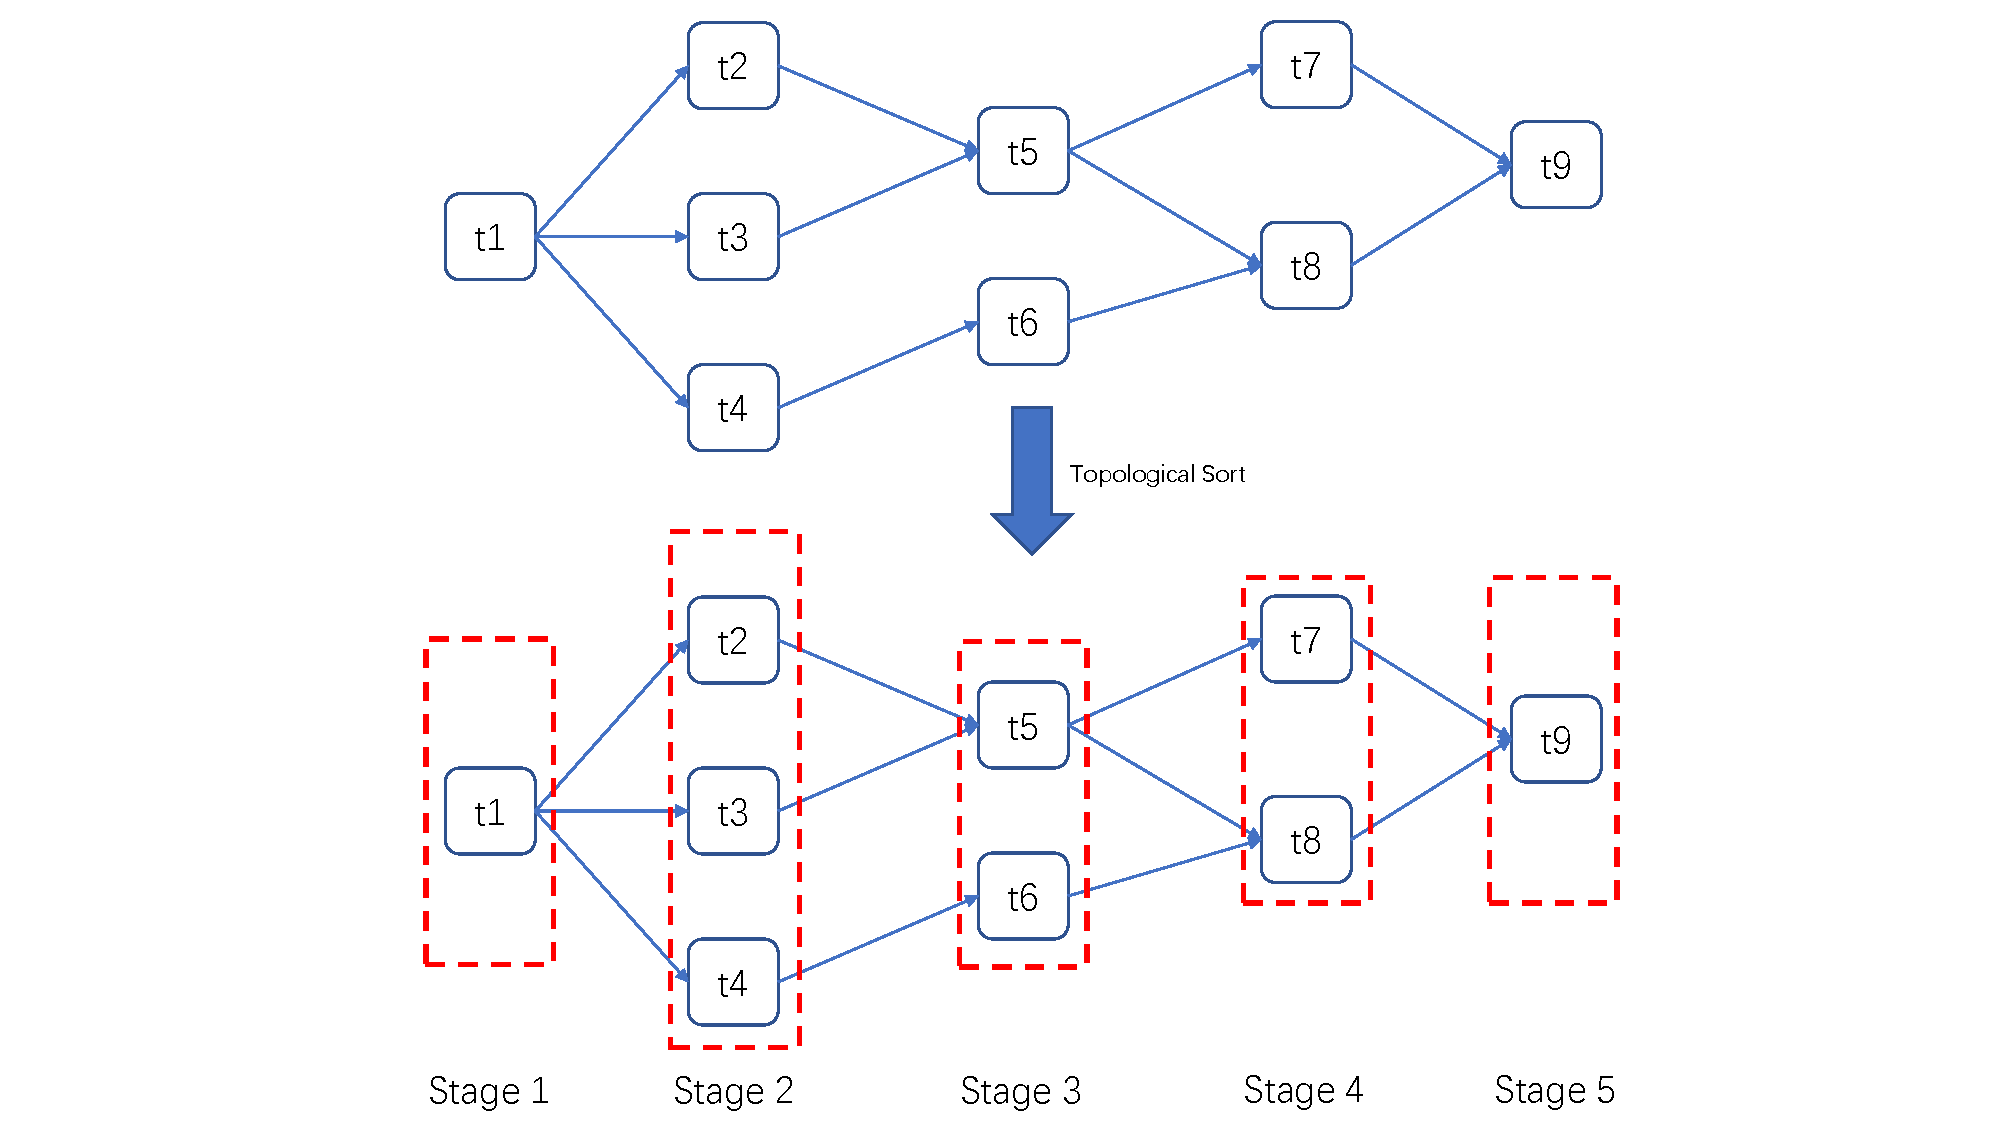
\includegraphics[width=15cm]{Figures/FigureDesign.pdf}
        \caption{Separating tasks into stages by topological sort}
        \label{fig:topological sort}
    \end{figure}
    \item We update the bandwidth between each data-center using the transfer station method, making sure that every pair of data-center is connected. The idea of this method is that if the bandwidth between two data-centers $A$ and $B$ is $0$, we may find a middle transfer station $C$, and the new bandwidth between $A$ and $B$ is $\min \left( bandwidth_{A\rightarrow C},bandwidth_{C\rightarrow B} \right) $. An example of the result of this method is shown in Fig. \ref{fig:transfer station}.
    \begin{figure}
        \centering
        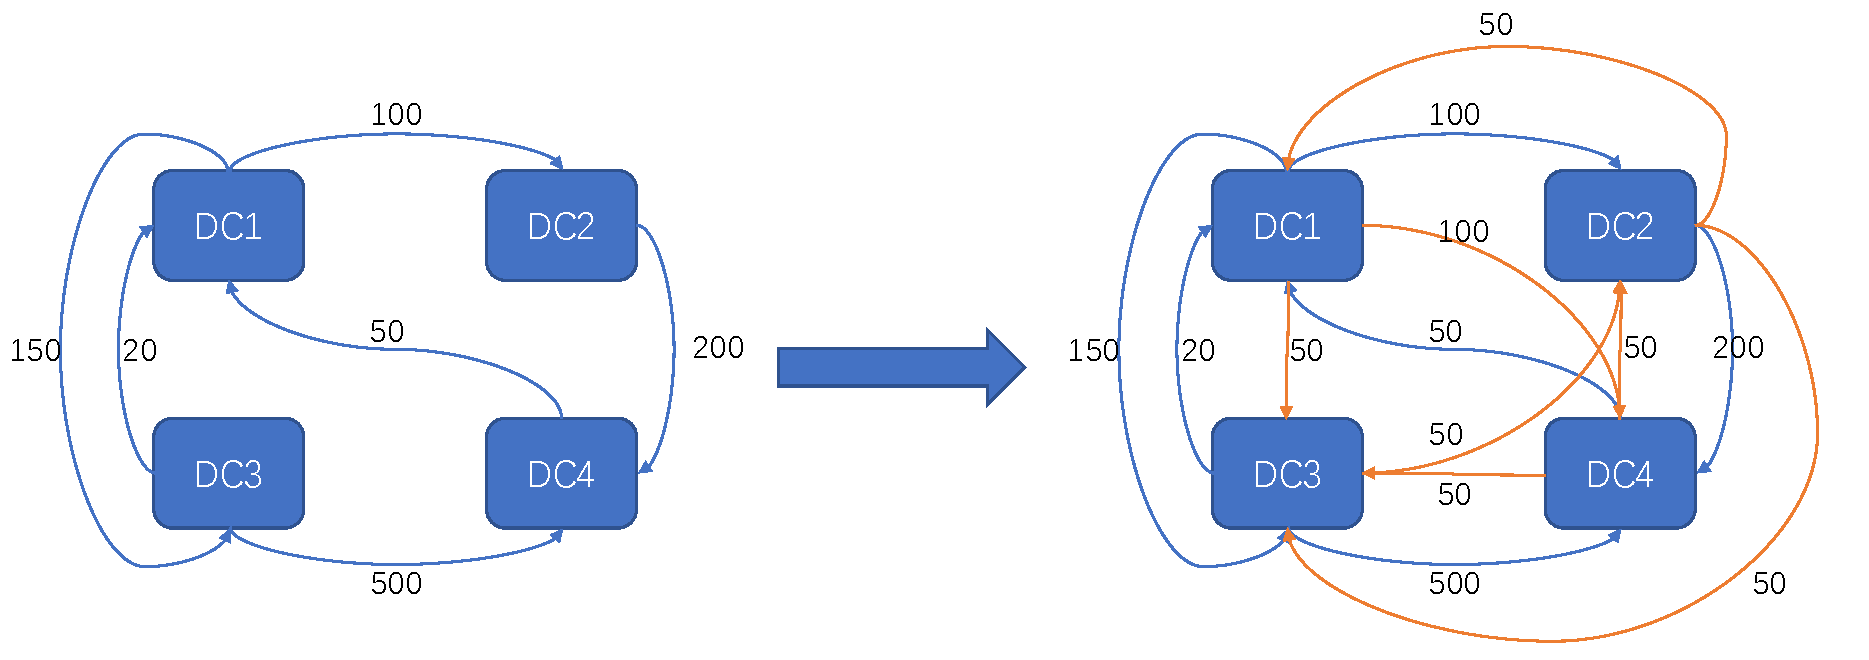
\includegraphics[width=15cm]{Figures/transfer_station.pdf}
        \caption{An example of updating bandwidth}
        \label{fig:transfer station}
    \end{figure}
\end{enumerate}

\section{Algorithm Design}
In this section, we first determine the constraints of the problem based on the analysis of data-set and requirements. 

Then, starting from a loose situation with fewer constraints, we gradually make the constraints more and more strict and respectively design $3$ algorithms for situations with different strictness.
\subsection{Loose Strictness: Genetic Algorithm (GA)}
\subsubsection{Brief Algorithm Introduction}
Since the scheduling problem has a very large feasible region, which is impossible to find the optimal solution in polynomial time, so we believe that using an algorithm to narrow the search space should be the first try.

After preliminary analysis, we find that the relatively good scheduling methods have some features in common. Therefore, our algorithm may be able to get the optimal solution by learning the features and generating better solutions by combining the features.

To learn and combine the features, the genetic algorithm (GA) may be an excellent method. Inspired by the process of natural selection, genetic algorithm is usually used to optimize a search problem relying on biologically inspired operators such as crossover, mutation and selection. 

During the evolution, the individuals of better solutions are more likely to survive due to higher fitness, and the next generation is generated by combining the gene of the alive individuals, which is exactly the procedure to learn and combine the features of good solutions.
\subsubsection{Encoding Method}
In order to transform each solution into the gene of an individual in the genetic algorithm, an encoding method should be figured out. 

The encoding method must satisfy the following rules:
\begin{enumerate}
\item
Each feasible scheduling method has a one-to-one correspondence with its gene.
\item
Genes are allowed to mutate without losing feasibility.
\item
A pair of genes can crossover with each other and generate new genes of feasible solutions.
\end{enumerate}

To satisfy the rules above, we encode each solution by the following procedure:
\begin{enumerate}
\item
For each task, encode the task with the ID of data-center it is processed
\item
For each job, create an array representing the processing location of its tasks
\item
Concatenate the arrays of all jobs into a long array, and this array is the gene of the scheduling method
\end{enumerate}

Here is an example to illustrate the encoding procedure:

Suppose there is two jobs: \textbf{A} and \textbf{B}. \textbf{A} consists two tasks: \textbf{tA1} and \textbf{tA2}, while \textbf{B} consists one task: \textbf{tB1}. And our scheduling method is depicted in Table \ref{tab:scheduling method}.
\begin{table}
    \centering
    \caption{Example of the scheduling method}
    \begin{tabular}{c|c|c}
        Job & Task & Data Center \\
          A & tA1  & DC1         \\
            & tA2  & DC3         \\
          B & tB1  & DC2         \\
    \end{tabular}
    \label{tab:scheduling method}
\end{table}
Then, our encoding procedure can be shown as follows:
$$
\begin{cases}
	A:\left[ 1,3 \right]\\
	B:\left[ 2 \right]\\
\end{cases}\Rightarrow \left[ \left[ 1,3 \right] ,\left[ 2 \right] \right] \xrightarrow{\mathrm{concatenate}}\left[ 1,3,2 \right] 
$$
\subsubsection{Simulation}
After encoding each scheduling method by a gene, we should design a way to decode each gene and execute the simulation of the real computation procedure. The simulation includes the following works:
\begin{enumerate}
    \item Firstly, we construct an Directed-Acyclic-Graph (DAG). 
    
    In the DAG, each node represents a task, the weight of which is the execution time of the task. Moreover, each edge represents the time needed to transfer data after the former task is done.
    \item Secondly, we separate the tasks into different stages using the topological sort. Then, we add a source node and a sink node on the beinning and end of the graph respectively.
    \item Eventually, to compute the finish time of each task, we only need to compute a finish time of each node by equation \ref{finish time}:
    \begin{equation}
        F_j=F_i+W_j+\max \left( E_{kj} \right)
        \label{finish time}
    \end{equation}
    Variables $F_i$, $W_i$ respectively means the finish time and the execution time of task $i$, while $E_{kj}$ means the weight of edge connecting task $k$ and $j$.
\end{enumerate}
\subsubsection{Optimization Method}
After decoding each gene and simulating the computation process, we are able to optimize the performance of the population.

Before the optimizing method we should first determine the goal. We are required to minimize the average completion time of all jobs while maintaining max-min fairness on computation resource.

After the analysis of the requirements, we think that our goal is minimizing the following two parts:
\begin{enumerate}
    \item Average completion time of all jobs, which is clearly required.
    \item The completion time if all jobs, since we believe that minimizing the total completion time satisfies the max-min fairness to some extent.
\end{enumerate}
Therefore, we design the fitness of the gene as equation \ref{fitness} shows, in which $T_i$ means the completion time of job $i$.
\begin{equation}
    fitness=\frac{1}{\mathrm{mean}\left( T_i \right) *\max \left( T_i \right)}
    \label{fitness}
\end{equation}
Then, by maximizing the fitness with GA, we could optimize the performance of gene.

\subsubsection{Complexity Analysis}
The complexity of the GA algorithm is the complexity of the optimization procedure.

Before the analysis, we define the meaning of symbols in Table \ref{tab:GA}
\begin{table}[]
    \centering
    \caption{Symbols used in the analysis of GA}
    \begin{tabular}{|c|c|}
    \hline
        {\bf Symbol} & {\bf Definition} \\ \hline
        $G$ & number of generation \\ \hline
        $P$ & population amount \\ \hline
        $L$ & length of gene \\ \hline
        $E$ & number of edges in the DAG \\ \hline
        $T_{func}$ & The time used to evaluate an individual's fitness \\ \hline
        $T_{opt}$  & The total time of the optimization procedure \\ \hline
    \end{tabular}
    \label{tab:GA}
\end{table}

The optimization is analyzed as following:
$$
T_{opt}=G\times \left[ P\times T_{func}+\left( P\times \log \left( P \right) +P^2 \right) +P\times L \right] 
$$

$P\times T_{func}$ represents the time used to evaluate the whole population, $P\times \log \left( P \right) +P^2$ is the time sort the individuals and select the individuals with higher fitness, and $P\times L$ means the time needed to crossover and generate the new generation.

Furthermore, we should also analyze the complexity of the fitness computation. When computing the fitness, we should traverse each edge in the DAG once and only once, which represents the data dependent. Therefore, the time complexity of fitness computation is $O(E)$.

All in all, the time complexity of the GA is:
$$
T_{opt}=O\left( G\times \left[ P\times E+\left( P\times \log \left( P \right) +P^2 \right) +P\times L \right] \right) =\begin{cases}
	O\left( G\times P^2 \right) , P\,\,\mathrm{is} \mathrm{relatively} \mathrm{large}\\
	O\left( P\times E \right) , E\,\,\mathrm{is} \mathrm{relatively} \mathrm{large}\\
	O\left( P\times L \right) , L\,\,\mathrm{is} \mathrm{relatively} \mathrm{large}\\
\end{cases}
$$





\subsection{Simulation: SJF and Random Optimization}

\subsubsection{Encoding Method}
We construct a task chain for each data center, and each task appears only once. For each task on the chain, only the task in front of the chain is completed, can the task be performed. In addition, before performing a task, it is necessary to ensure that the task's pioneer tasks are completed and that the current data center slot is not full. The following two tables shows this encoding method. In particular, these two encoding methods all belongs to the optimal coding for toy-data(17.65s).

\begin{minipage}[t]{0.45\textwidth}
\fbox{%
  \parbox{\textwidth}{%
 \rm DC1 : tB1 $\rightarrow$ tE4 $\rightarrow$ \\
 \rm DC2 : tD4 $\rightarrow$ tE2 $\rightarrow$ tF8 $\rightarrow$ \\
 \rm DC3 : tD3 $\rightarrow$ tF3 $\rightarrow$ tF2 $\rightarrow$ \\
 \rm DC4 : tC1 $\rightarrow$ tD5 $\rightarrow$ tC3 $\rightarrow$ \\
 \rm DC5 : tE1 $\rightarrow$ tE5 $\rightarrow$ \\
 \rm DC6 : \\
 \rm DC7 : tD1 $\rightarrow$ tE3 $\rightarrow$ tF6 $\rightarrow$ tF7 $\rightarrow$ \\
 \rm DC8 : tC2 $\rightarrow$ tF4 $\rightarrow$ tF5 $\rightarrow$ \\
 \rm DC9 : tD2 $\rightarrow$ tE6 $\rightarrow$ \\
 \rm DC10 : \\
 \rm DC11 : \\
 \rm DC12 : tA2 $\rightarrow$ tB2 $\rightarrow$ \\
 \rm DC13 : tF1 $\rightarrow$ tA1 $\rightarrow$ tF9 $\rightarrow$
  }%
}
\end{minipage}
\hfill
\begin{minipage}[t]{0.45\textwidth}
\fbox{%
  \parbox{\textwidth}{%
 \rm DC1 : tF5 $\rightarrow$ tF9 $\rightarrow$ \\
 \rm DC2 : tD2 $\rightarrow$ tD3 $\rightarrow$ \\
 \rm DC3 : tD4 $\rightarrow$ \\
 \rm DC4 : tD1 $\rightarrow$ tE6 $\rightarrow$ \\
 \rm DC5 : tE1 $\rightarrow$ tE3 $\rightarrow$ \\
 \rm DC6 : tE2 $\rightarrow$ tE5 $\rightarrow$ \\
 \rm DC7 : tA2 $\rightarrow$ tF4 $\rightarrow$ \\
 \rm DC8 : tA1 $\rightarrow$ tF6 $\rightarrow$ \\
 \rm DC9 : tF1 $\rightarrow$ tC2 $\rightarrow$ tF8 $\rightarrow$ \\
 \rm DC10 : tF3 $\rightarrow$ tC3 $\rightarrow$ \\
 \rm DC11 : tC1 $\rightarrow$ tB1 $\rightarrow$ tE4 $\rightarrow$ \\
 \rm DC12 : tB2 $\rightarrow$ tF2 $\rightarrow$ tD5 $\rightarrow$ \\
 \rm DC13 : tF7 $\rightarrow$ 
  }%
}
\end{minipage}

\subsubsection{Algorithm Design}
In this part, we use two strategies: random optimization algorithm and short job first strategy. We introduce our task simulator firstly. 

For the \textbf{simulator}, we set up a time heap for each data center and construct an event heap globally. To simulate programmed task chains, we traverse each data center. Every DC has a pointer pointing to the current task to be finished. If the current data center slot is not full and all the pioneer tasks are completed, then the data will be taken and the task will be executed. In the global event heap, we build the heap according to the sequence of events. Every time a task starts to execute, we add the end event to the event heap. If all data centers have no tasks to run, then go to the top of the event heap to get an event, set the current time to the event time and reduce the in-degree of subsequent tasks by one. If the global task heap is empty and all the DC's pointers have moved to the last place, then we believe that all tasks have been carried out. Otherwise, we call we meet a simulator deadlock.

\begin{algorithm}

\BlankLine
\caption{Simulate Algorithm}
\label{alg:simu}
\BlankLine
eventHeap $\leftarrow$ []

\While{\rm \textbf{True}}{
    executed $\leftarrow$ {\rm \textbf{False}}
    
    \For{\rm dataCenter {\rm \textbf{in}} dataCenterList}{
    \rm
        executed $\leftarrow$ dataCenter.runOneTask(eventHeap) \textbf{or} executed
    }
    
    \If{\rm \textbf{not} executed}{
        \If {\rm len(eventHeap) == 0}{
            finished $\leftarrow$ \textbf{True}
            
            \For{\rm dataCenter \textbf{in} dataCenterList}{
                \If{\rm \textbf{not} dataCenter.finished}{
                    finished $\leftarrow$ \textbf{False}

                    \break
                }
            }

            \Return{\rm (finished, currentTime)}
        }
        event $\leftarrow$ heapq.heappop(eventHeap)
        
        \For{\rm e \textbf{in} next(event)}{
            $\rm e.indegree--$
            
            \If{\rm e.indegree == 0}{
                e.ready $\leftarrow$ \textbf{True}
            }
        }
        
        currentTime $\leftarrow$ event.time
        
    }
}
\end{algorithm}

For the \textbf{random optimization algorithm}, we first generate the task code randomly. Next, we perform the simulation and do two kinds of optimization. If the task pointed to cannot be executed, but there is a task behind on the task chain that can be executed, then swap the two and execute the task that was changed to the front. For some two DCs, we can also schedule the tasks at the end of one's task chain to another for execution.

For the \textbf{SJF strategy}, we not only set the event heap, but also set a global ready heap to put ready tasks into it. For any event, there are \#DC editions in the ready heap to record the required time the task to be completed in each DC. We sort the events according to the required time in ready heap. In each iteration, we go to the top of the ready heap to pick up a task that has the shortest required time, and then register the end event in the event heap. When ready heap is empty or all DCs are full, take an event from event heap to update the global time.

\subsubsection{Complexity Analysis}
We claim that the complexity of simulation algorithm is $\Theta(|J|n\log n)$, because during each round of traversal the DCs will complete at least one task. The storage operation of heap needs logarithmic event complexity. In the worst case, every two rounds of traversal will encounter a case of no event execution. Then the complexity is also $\Theta(|J|n\log n)$ because the pop operation's complexity is also in logarithmic.

We claim that the complexity of SJF is $\Theta(|J|^2 n\log (|J|n))$. Because in this case every task has $\rm |J|$ version in the heap, so we need to replace $n$ with $n|J|$ in ``$\Theta(|{J}|n\log n)$".
          

\subsection{Strict Situation: Linear Programming (LP)}
\subsubsection{Optimizing the Worst Completion Time among Concurrent Jobs}
Our target~\ref{eq:target1} is a vector optimization with multiple objectives. To have a more simple and intuitive overview of the problem, here we consider the single-objective sub-problem of optimizing the worst job performance as following:
\begin{equation*}
    \begin{aligned}
    \mbox{min}_x \quad &\mbox{max}_{k \in \mathcal{K}}(\tau_k) \\
\mbox{s.t.} \quad &\mbox{Constraints~\ref{eq:con1},~\ref{eq:con2},~\ref{eq:con3} and~\ref{eq:con4}.}
    \end{aligned}
\end{equation*}

Replacing the completion time $\tau_k$ in the objective with Equation~\ref{eq:con1}, we could induce the following problem with totally linear constraints:
\begin{equation}
    \begin{aligned}
    \mbox{min}_x \quad &\mbox{max}_{k \in \mathcal{K}}(\mbox{max}_{i \in \mathcal{T}_k, j \in \mathcal{D}} x_{i,j}^k(c_{i,j}^k+e_{i,j}^k)) \\
\mbox{s.t.} \quad &\mbox{Constraints~\ref{eq:con2},~\ref{eq:con3} and~\ref{eq:con4}.} 
    \end{aligned}
    \label{eq:target2}
\end{equation}

However, this typical ILP problem is still not that easy to be solved since it has a complex min-max-max objective, and the integer formular is not that friendly for Solvers like {\bf Gurobipy}.

Fortunately, reference \cite{ref_11} tells us that our problem has beautiful mathematical properties of separable convex objective and totally unimodular linear constraints. Exploiting these two properties, we can use the $\lambda$-representation \cite{ref_11} technique to transform Problem~\ref{eq:target2} into a linear programming problem that has the same optimal solution:
\begin{equation}
    \begin{aligned}
    \mbox{min}_{x,\lambda} \quad &\sum_{k \in \mathcal{K}} \sum_{i \in \mathcal{T}_k}\sum_{j \in \mathcal{D}}(\lambda_{i,j}^{k,0}+M^{c_{i,j}^k+e_{i,j}^k}\lambda_{i,j}^{k,1}) \\
\mbox{s.t.} \quad &x_{i,j}^k=\lambda_{i,j}^{k,1}, \forall k \in \mathcal{K}, i \in \mathcal{T}_k, j \in \mathcal{D} \\
&\lambda_{i,j}^{k,0}+\lambda_{i,j}^{k,1}=1, \forall k \in \mathcal{K}, i \in \mathcal{T}_k, j \in \mathcal{D} \\
&\lambda_{i,j}^{k,0},\lambda_{i,j}^{k,1},x_{i,j}^k \in \mathbb{R^+}, \forall k \in \mathcal{K}, i \in \mathcal{T}_k, j \in \mathcal{D} \\
&\mbox{Constraints~\ref{eq:con2} and~\ref{eq:con3}.} 
    \end{aligned}
    \label{eq:target3}
\end{equation}

Here $M = J\sum_{k=1}^K n_k$, where $J$ is the total number of the datacenters, while $n_k$ is the total number of tasks in job $k \in \mathcal{K}$. $\lambda_{i,j}^{k,0}$ and $\lambda_{i,j}^{k,1}$ are newly introduced variables to avoid $x$'s integrity (it's magical that this problem's solution will always yiled $x_{i,j}^k$ between 0 or 1).

Solving the above problem with Solvers like Gurobipy, we could achieve the minimum worst job completion time among all jobs.

\subsubsection{Iteratively Optimizing Worst Completion Times To Achieve Max-Min Fairness}
With the sub-problem of minimizing the worst completion time efficiently solved as an LP problem, we could continue to solve the original lexicographical minimization problem by minimizing the next worst completion time iteratively.

Our basic strategy is intuitive: After solving the sub-problem, if we find that the optimal worst completion time is achieved by a certain job $k^*$, we could fix all of its tasks, remove them from the equations, update the state variables,  then start the next iteration. All tasks of job $k^*$ could be removed because one job's completion time is determined by its longest task, as it has already been minimized, there is no need to consider other of its tasks. Hence, we could concentrate on the other jobs' tasks:
\begin{algorithm}
\KwIn{Job Set $\mathcal{K}$, input data sizes $d_i^{k,s}$ and link bandwidth $b_{s,j}$ to obtain network transfer time $c_{i,j}^k$; execution time $e_{i,j}^k$; data-center resource capacity $a_j$}
\KwOut{Task assignment $x_{i,j}^k,\forall k \in \mathcal{K}, \forall i \in \mathcal{T}_k, \forall j \in \mathcal{D}$}
\BlankLine
\caption{Optimal Assignment among Jobs with Max-Min Fairness}
\label{alg:basicLP}
\BlankLine
Initialize $\mathcal{K'}=\mathcal{K}$; \\
\While{$\mathcal{K'} \neq \varnothing$}{
    Solve the LP Problem~\ref{eq:target3} to obtain the solution $\bold{x}$; \\
    Obtain $\tau_{k^*}=\mbox{argmax}_{k \in \mathcal{K}} \tau_k$; \\
    Fix $x_{i,j}^{k^*}, \forall i \in \mathcal{T}_{k^*}, \forall j \in \mathcal{D}$; remove them from variable set $\bold{x}$; \\
    Update the corresponding resource capacities in Constraints; \\
    Remove $k^*$ from $\mathcal{K'}$;
}
\Return{$\bold{x}$};
\end{algorithm}

As a result, we will minimize the $i$th longest job completion time after the $i$th iteration, the max-min fairness could be achieved when Algorithm~\ref{alg:basicLP} terminates.

\subsubsection{Scheduling Jobs In a DAG}
In real life, however, there would be more constraints within a job, for example, the precedence. As shown in Fig.~\ref{fig:topological sort}, a job could be represented by a DAG, where each directed edge indicates a precedence constraint. To make the scheduling problem more convenient and practical to be solved, we use {\bf Topological Sort} to divide the tasks into stages, and add constraint that all tasks among the same stage could run in parallel after all its former stages have been completed. Now the problem comes that how should we scheduler between stages to achieve a more reasonable job completion time while maintaining the max-mix fairness.

Our basic idea is to maintain a {\bf scheduling pool}. It's not wise to reschedule all the tasks when a certain stage of a job has been finished. From the algorithm's perspective, it could raise a high time complexity. Besides, it's also not practical to move a running task to another computing slot. 

So we develop Algorithm~\ref{alg:DAG} to deal with DAG-Jobs scheduling: We will push the tasks in the next stage into the scheduling pool when a certain stage has finished. And as we've discussed above, we'll only schedule the newly coming tasks. Under consideration of multiple factors, for example, to reduce time complexity, or to get more available computing slots during the scheduling, we set two thresholds to trigger a new scheduling: the job number threshold $ts_{job}$ and the time threshold $ts_{time}$.  When the jobs in the scheduling pool has exceeded $ts_{job}$ or the time from last scheduling has exceeded $ts_{time}$, a new round of scheduling will be triggered. 
\begin{algorithm}
\KwIn{DAG-Job set $\mathcal{K}$, time threshold $ts_{time}$,  job threshold $ts_{job}$ and the same input as Algorithm~\ref{alg:basicLP}}
\KwOut{Task assignment $x_{i,j}^{k},\forall k \in \mathcal{K}, \forall i \in \mathcal{T}_k, \forall j \in \mathcal{D}$}
\BlankLine
\caption{DAG-Jobs Scheduler}
\label{alg:DAG}
\BlankLine
Current time $t \leftarrow 0$; \\
Task Assignment $\bold{x} \leftarrow \varnothing$;
Initialize $\mathcal{K'}=\mathcal{K}$; \\
Push all tasks in stage 1 into the scheduling pool; \\
\While{$\mathcal{K'} \neq \varnothing$}{
    Run Algorithm~\ref{alg:basicLP} (and Algorithm~\ref{alg:Serial}) for all tasks in scheduling pool to get $\bold{x'}$; \\
    Push $\bold{x'}$ into $\bold{x}$; \\
    Sort all job finishing time in current stage in ascending order to get $\bold{\tau}$; \\
    Wait time $t_{wait} \leftarrow 0$; \\
    \For{$i \leftarrow 1 \ \mbox{to} \ ts_{job}$}{
        $t_{wait} \leftarrow \tau[i] - t$; \\
        \If{$t_{wait} > ts_{time}$}{Break;}
        \Else{$t \leftarrow \tau[i]$;\\
        \If{All the stages in job $i$ has been finished}{Remove $i$ from $\mathcal{K'}$}
        \Else{Push all the tasks in job $i$'s next stage into the scheduling pool;}        
        }
    }
}
\end{algorithm}

\subsubsection{Optimization In Serial Execution}
Though the introduced algorithm could already achieve a reasonable and effective solution under most of situations, it could still suffer when encountering some extreme situations. One of the situation could be shown as below:
\begin{figure}[htbp]
    \centering
    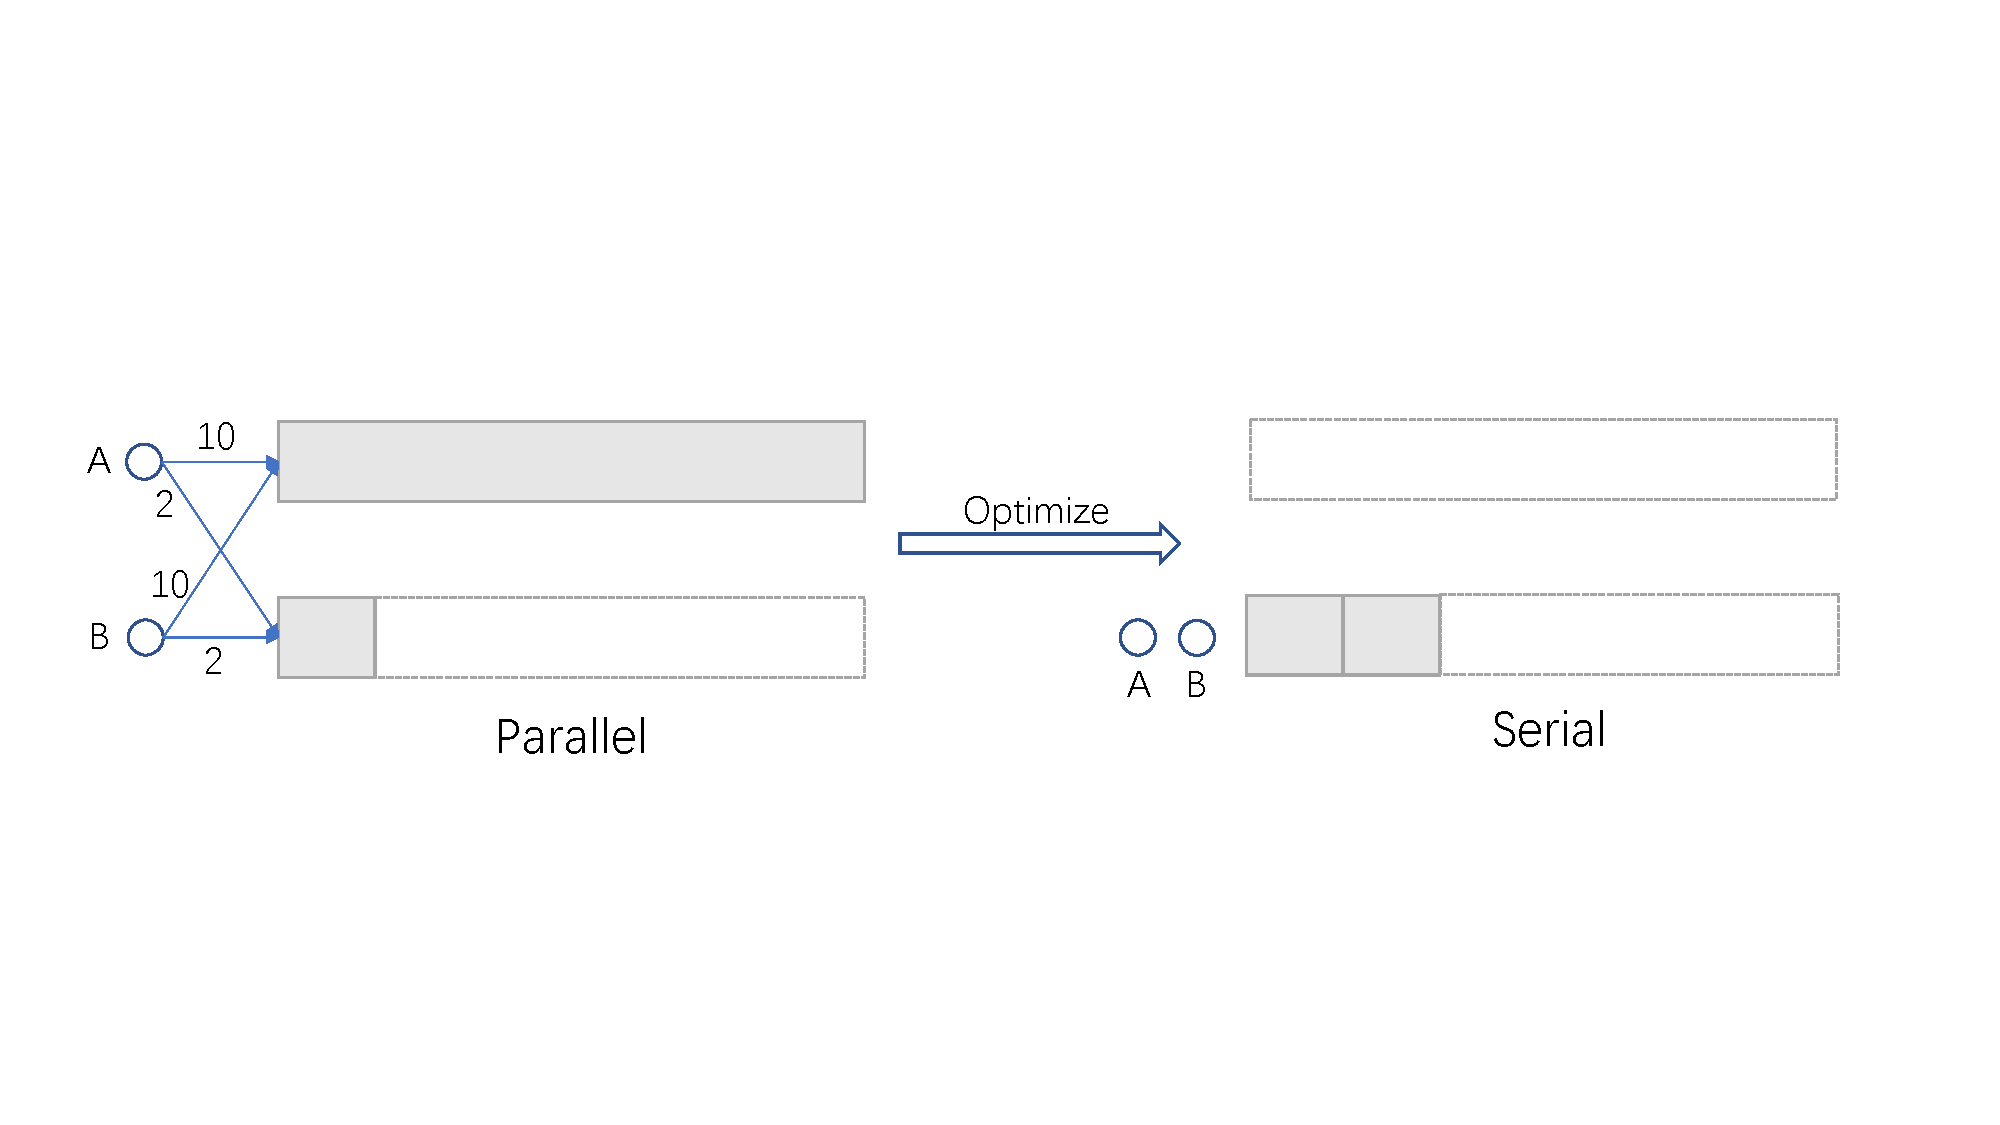
\includegraphics[width=0.8\textwidth]{Figures/CounterExample.pdf}
    \caption{Parallel Counter Example}
    \label{fig:CounterExp}
\end{figure}

The key problem is that sometimes a serial running sequence could be better than running in parallel, for example, when we have a supercomputer that beats all the other machines in performance.

To deal with this problem without prejudice to LP's transformation constraints, we simply add some condition check after running Algorithm~\ref{alg:basicLP}. Additionally, we should maintain every task's completion time during execution.

After all the tasks have been set, we'll look back onto the longest time task in each job. It may have a better place to be computed, but haven't been scheduled into it due to the number of slots is finite. So we traverse all the data-centers and try to assign the task into it after a certain task has finished and a slot has been available again. Adding up the extra waiting time, if the newly serial execution time is still less than what we've scheduled before, we'll reschedule the task into the newly found data-center.
\begin{algorithm}
\KwIn{Current Task Assignment $\bold{x}$, current task finishing time $\bold{t}$, network transfer time $\bold{c}$, data-center set $J$}
\KwOut{Updated Task Assignment $\bold{x}$, updated task finishing time $\bold{t}$}
\BlankLine
\caption{Serial Optimizer}
\label{alg:Serial}
\BlankLine
Find the bottleneck task for each job $k \in \mathcal{K}$ to get $bottle\_task$; \\
\For{task $i$ in $bottle\_task$}{
    $j^* \leftarrow current \ assigned \ location$; \\ 
    \For{$j$ in $J$}{
            Find the next task finishing time $t$ in datacenter $j$; \\
            \If{$t+c_{i,j}^k < c_{i,j^*}^k$}{
                Reallocated task $i$ to datacenter $j$ after that task has finished; \\
                Update $\bold{x}$ and $\bold{t}$;
            }
    }
}
\Return{$\bold{x}, \bold{t}$}
\end{algorithm}

The scheduler's general structure is shown in Fig.~\ref{fig:Structure}. Now the scheduling algorithm is more robust and could give more reasonable solutions under extreme situations.
\begin{figure}[htbp]
    \centering
    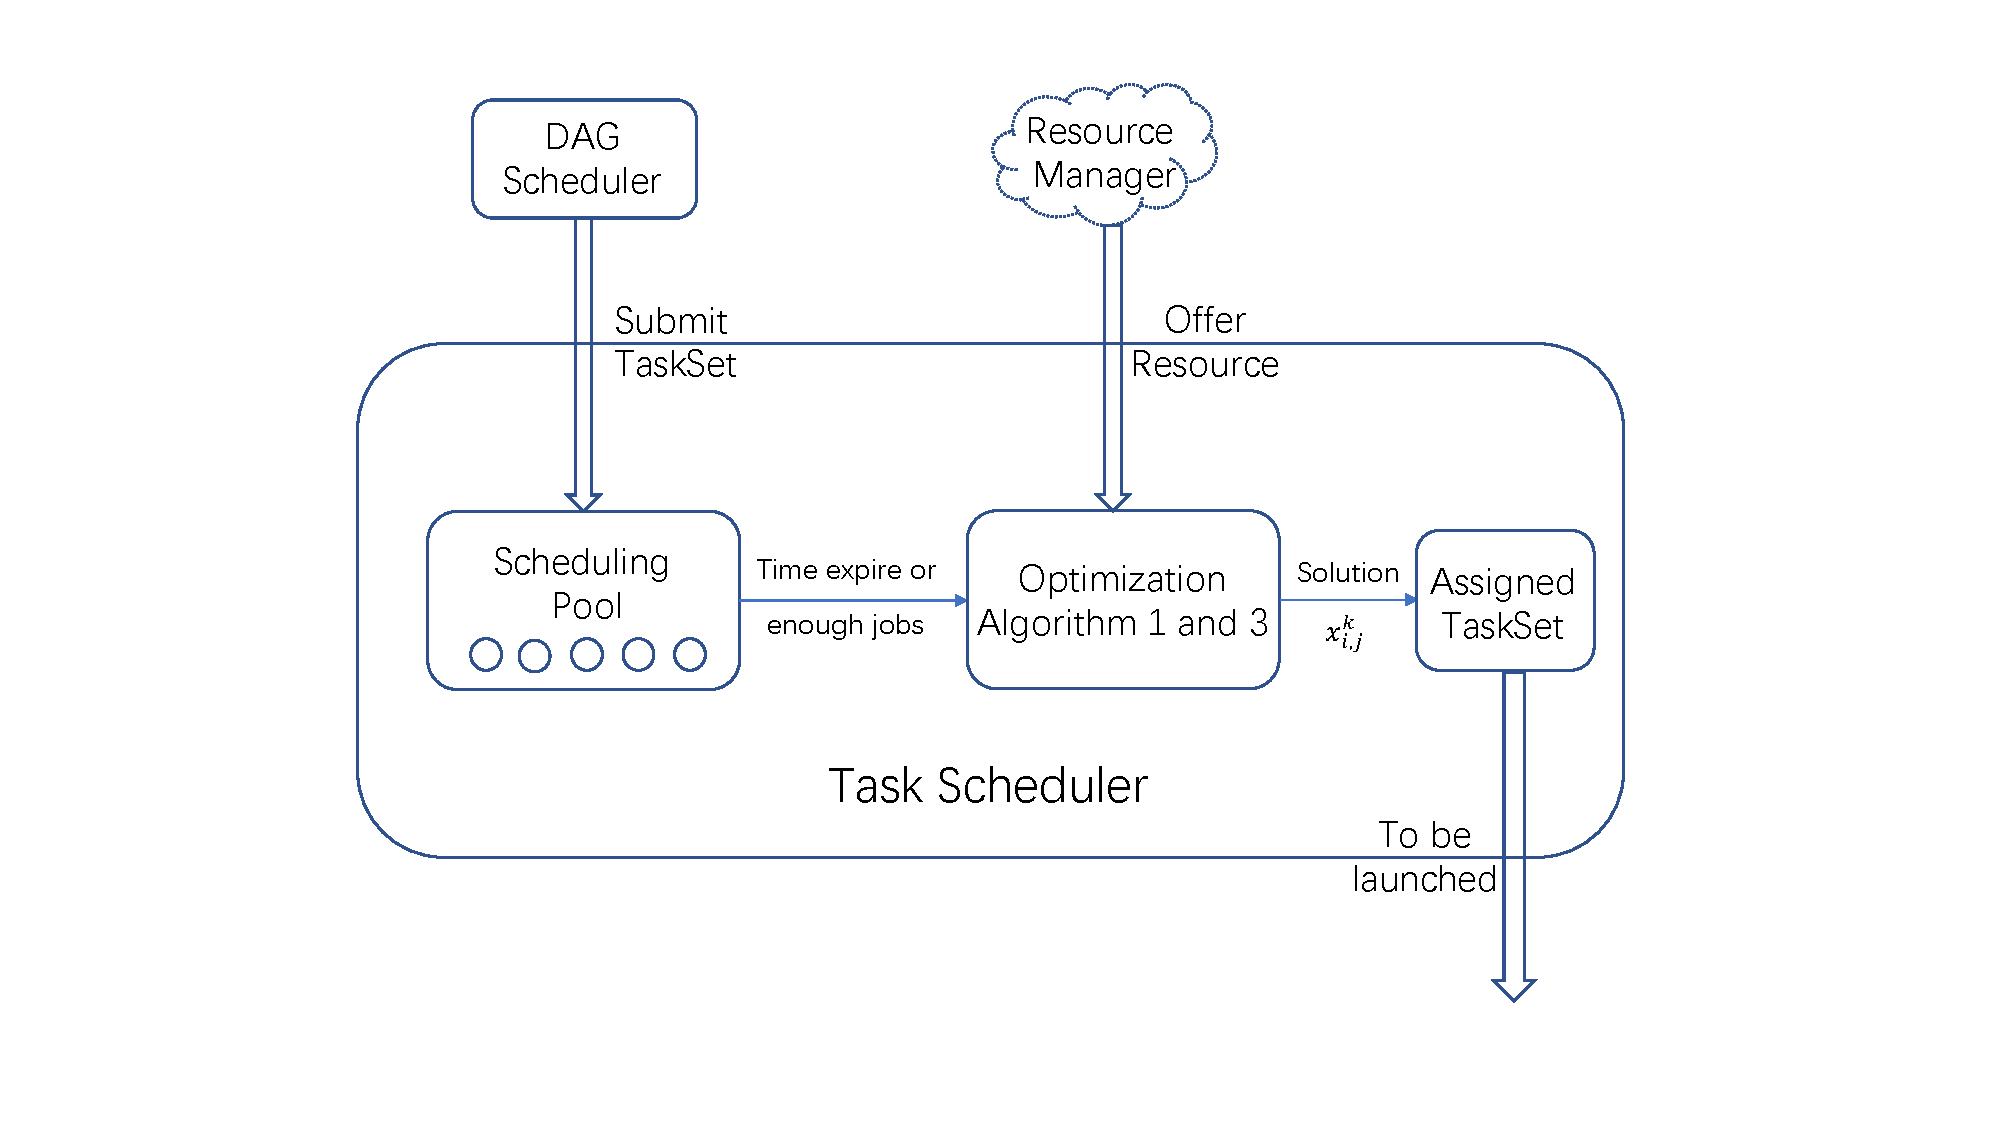
\includegraphics[width=0.8\textwidth]{Figures/SchedulerStructure.pdf}
    \caption{Scheduler Structure}
    \label{fig:Structure}
\end{figure}

\subsubsection{Complexity Analysis}
\;

{\bf First}, for the space complexity. Suppose we have $K$ jobs, each with $\mathcal{T}_k$ tasks, and $J$ datacenters. Our algorithm helps to find $x_{i,j}^k$, that is, the task assignment locations. Let $N_K = \sum_{i=1}^K \mathcal{T}_k$ denote the total number of tasks, we use extra $O(N_K \times J)$ space to store the variables. Besides, we also store matrix such as $c_{s,j}$, which is $O(J^2)$, normally smaller than $O(N_K \times J)$. So after all, the LP Algorithm's space complexity is $O(N_K \times J)$.

{\bf Second}, for the time complexity. Taking an eye on Algorithm~\ref{alg:DAG}, the main body is a while loop which will run until all the job has been finished. However, inside the loop Algorithm~\ref{alg:basicLP} and Algorithm~\ref{alg:Serial} will be triggered at random. Here we simply considering the job threshold, suppose each $\mathcal{T}_k$ job has $O(log(\mathcal{T}_k))$ stages. Let $S_K = \sum_{i=1}^K log(\mathcal{T}_k)$ denote the number of total stages, then the while loop will run $O(S_K)$ times.

Inside each loop, the main time cost is risen from Algorithm~\ref{alg:basicLP}. Reasonably, we ignore all the update operations in Algorithm~\ref{alg:basicLP} and concentrate on Line 3: Solving the LP problem. If we use {\bf Simplex} method to solve the LP problem, then according to \cite{ref_13}, it has a polynomial average complexity of number of variables and constraints, which is $O(N_K^L)$, while the worst time complexity is of exponential time $O(2^{N_k})$.

So after all, the LP Algorithm has a average time complexity of $O(S_K \times N_K^L)$ (polynomial) while the worst is $O(S_K \times 2^{N_k})$ (exponential).

\section{Test on Toy-Data (Small Data)}
In this section, we run our algorithms on the given toy data-set to test their correctness. Besides, in order to have a deeper insight of our algorithms, we randomly generate data to conduct more comparing-experiments, we also list their results here.
\subsection{Toy Data Analysis}
\subsubsection{Results Overview}
The given toy data-set has 6 jobs to be scheduled in 13 different data-centers, each has several states which should be executed in sequence. After running our three algorithms on it, we get following results:
\begin{table}[htbp]
    \caption{Toy-Data Experiment Results}
    \centering
    \begin{tabular}{|c|c|c|c|}
    \hline
       {\bf Algorithm} &{\bf Worst JCT (s)} &{\bf Average JCT (s)} &{\bf Running Time (s)} \\ \hline
       Baseline &29.28 &12.44 &/ \\ \hline
       LP &22.62 &9.83 &0.33 \\ \hline
       GA &17.65 &7.20 &1.02 \\ \hline
       SJF &17.75 &7.31 &0.701 \\ \hline
    \end{tabular}
    \label{tab:toyResults}
\end{table}

In a nutshell, all our three algorithms have much better performance over the baseline (which is generated in the first iteration of GA). However, different algorithms seem to have different running time and task assignment strategies.

As we've discussed above, LP tends to satisfy tight constraints (like lexicographic order) in every iteration. Besides, it still has defects of less serial execution, so it may not give out an optimal solution. However, thanks to the solver {\bf Gurobipy}, LP is the fastest algorithm among the three as well as yielding a reasonable result. The Genetic Algorithm runs a bit slower, however, it gives out the best assignment, so it makes sense when we need to find an optimal scheduling. Finally, the SJF is a median of running time and assignment, which is also a great choice when we have limited computing resource.

The best case (17.65s) task assignment state is shown in Fig.~\ref{fig:bestAssign}.
\begin{figure}[htbp]
    \centering
    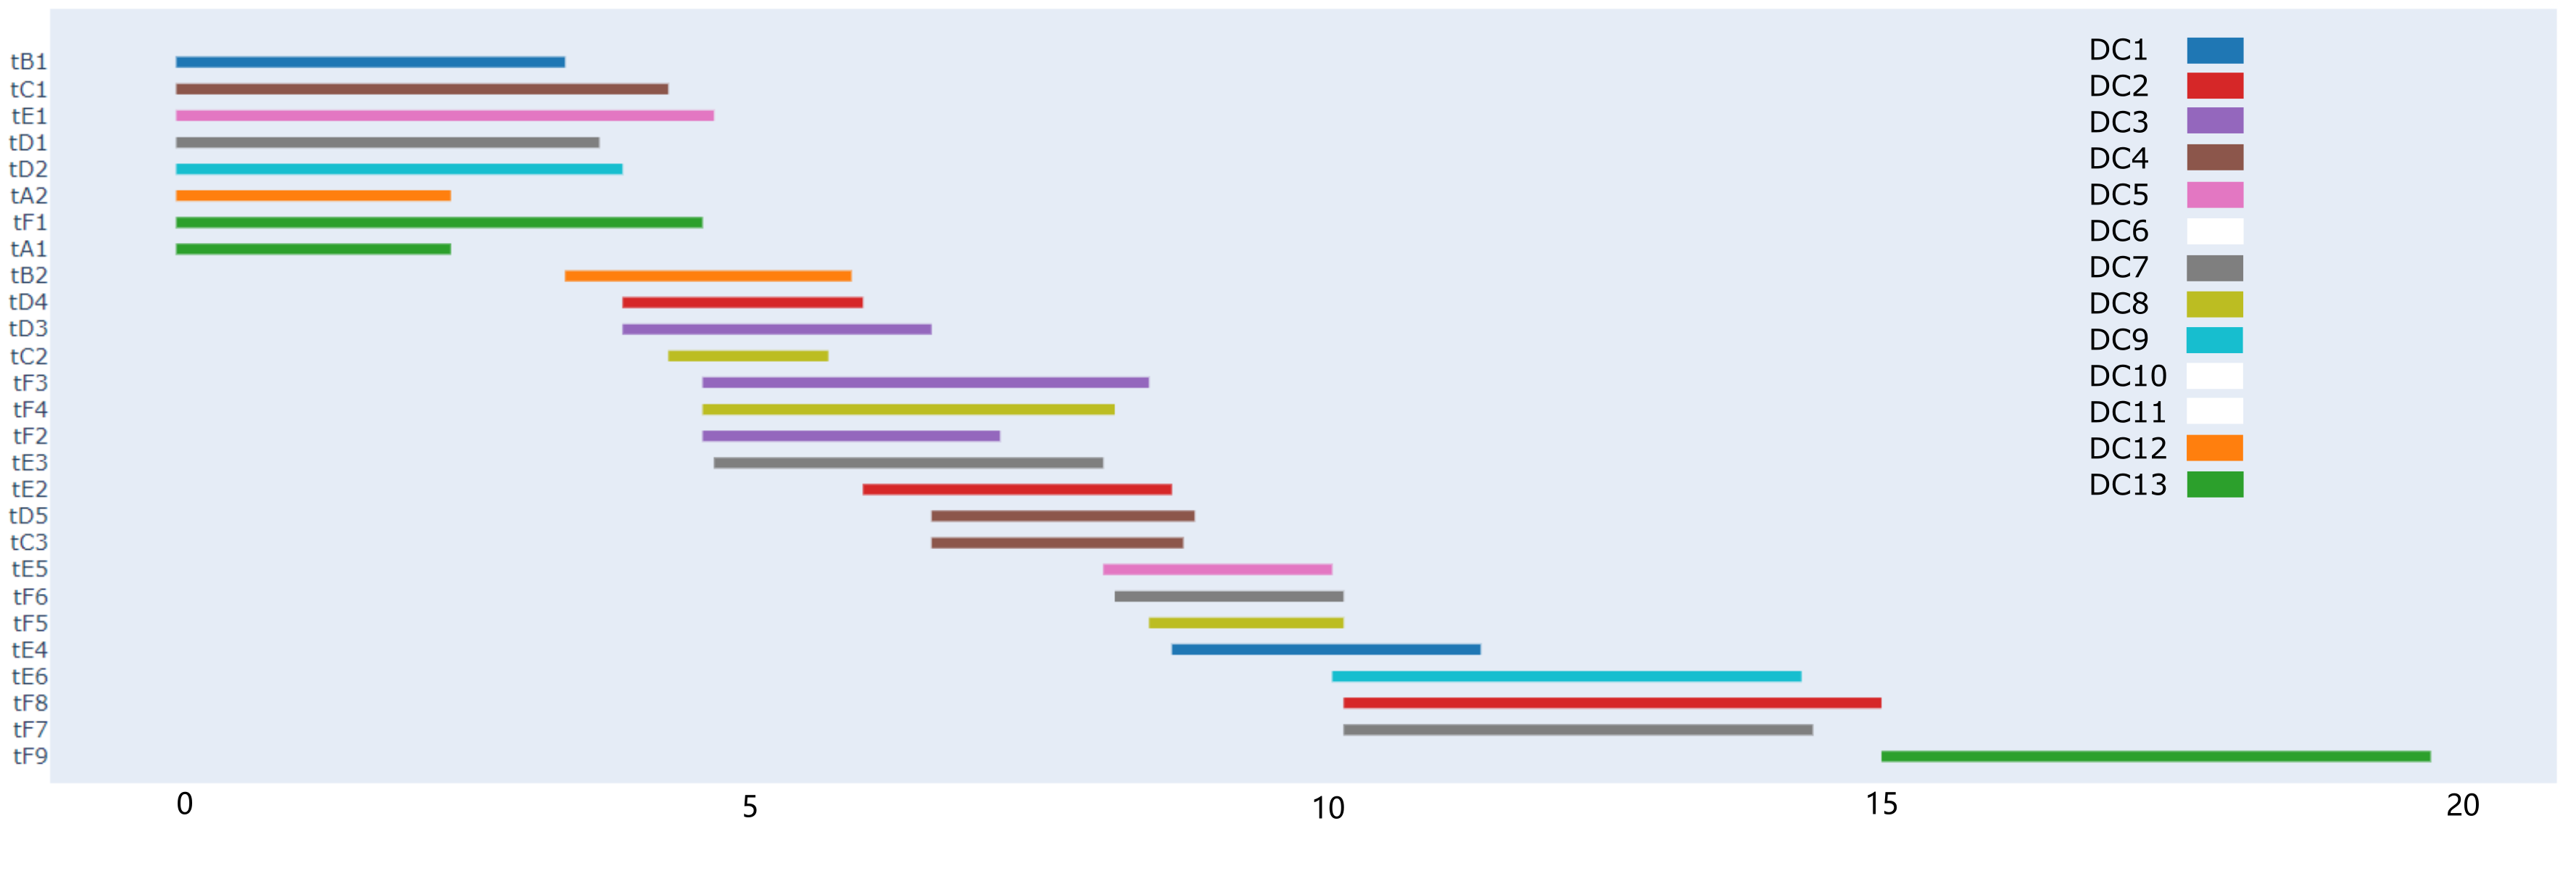
\includegraphics[width=0.8\textwidth]{Figures/gannt.png}
    \caption{Best Case Task Assignment}
    \label{fig:bestAssign}
\end{figure}

\subsubsection{GA Optimization Procedure}
Typically, we unfold GA's optimization procedure in this subsection. 

We initialized 10000 individuals as the initial population, and then optimized it according to the genetic algorithm.

During the optimization procedure, The fitness of the best individual and the average fitness both increase gradually, as shown in Fig. \ref{fig:fitness}.
\begin{figure}
    \centering
    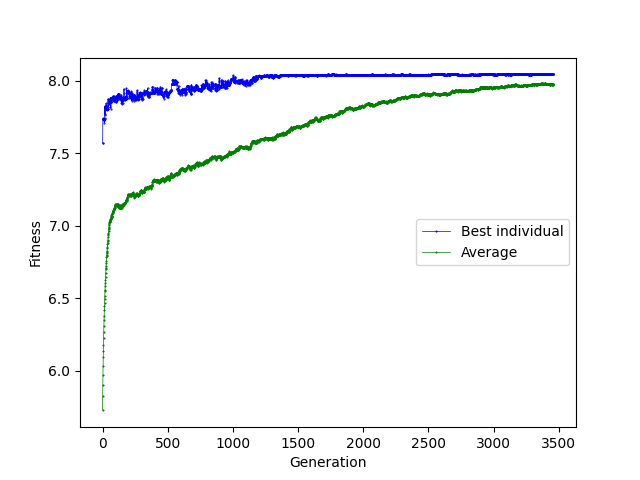
\includegraphics[width=0.8\textwidth]{Figures/fitness.png}
    \caption{Evolution of Fitness}
    \label{fig:fitness}
\end{figure}

Moreover, we found that in the optimization process, the value of each segment of the gene tends to eventually converge to a certain value or a few values, so we drew a heat map of the value of the gene in the optimization process. This means that the algorithm does learn the features of the better solutions and successfully maintain the features.

The heat map of generation $0$, $5$, $20$, $100$, $1000$ and $3000$ is shown from Fig. \ref{fig:g0} to Fig. \ref{fig:g3000}.

The abscissa in the heat map represents the fragment of the gene, while the ordinate represents the value, and the color depth represents the number of times this value is taken.

\begin{figure}[htbp]
\centering
\begin{minipage}[t]{0.3\linewidth}
\centering
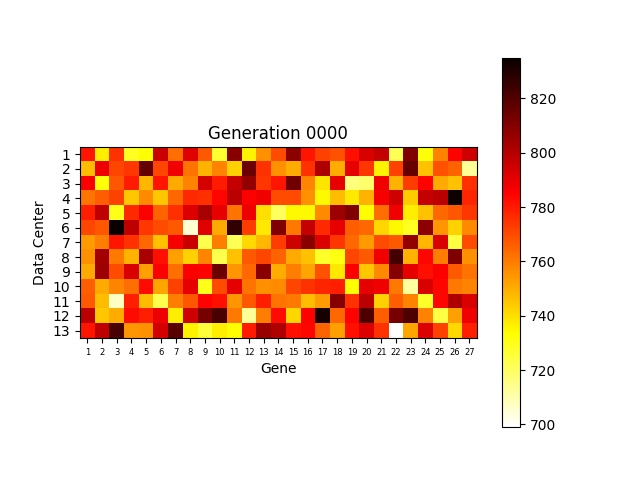
\includegraphics[width=5cm]{Figures/Generation 0000.jpg}
\caption{Generation 0}
\label{fig:g0}
\end{minipage}
\begin{minipage}[t]{0.3\linewidth}
\centering
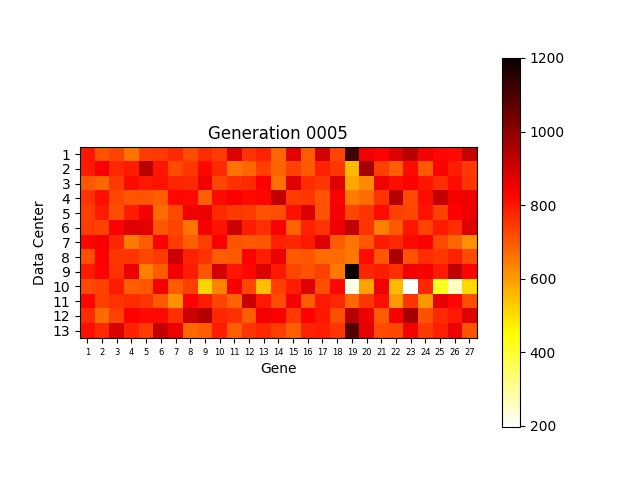
\includegraphics[width=5cm]{Figures/Generation 0005.jpg}
\caption{Generation 5}
\label{fig:g5}
\end{minipage}
\begin{minipage}[t]{0.3\linewidth}
\centering
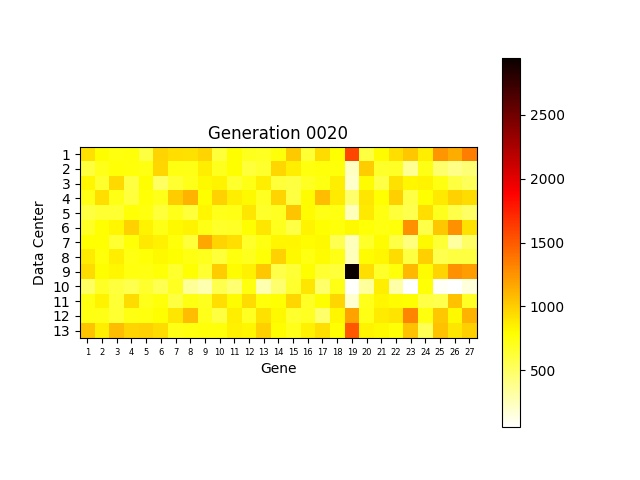
\includegraphics[width=5cm]{Figures/Generation 0020.jpg}
\caption{Generation 20}
\label{fig:g20}
\end{minipage}
\end{figure}

\begin{figure}[htbp]
\centering
\begin{minipage}[t]{0.3\linewidth}
\centering
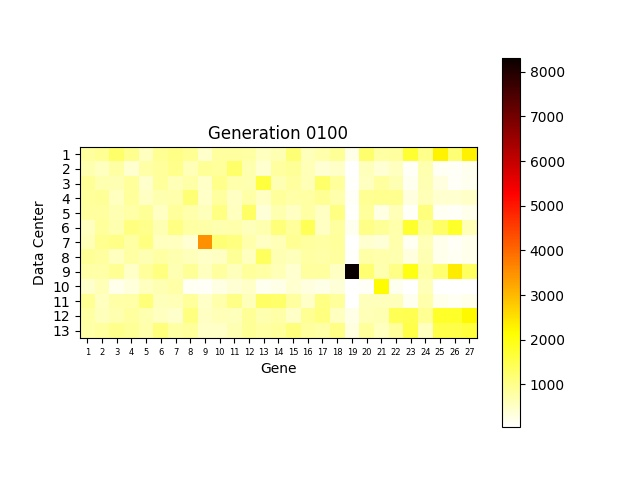
\includegraphics[width=5cm]{Figures/Generation 0100.jpg}
\caption{Generation 100}
\label{fig:g100}
\end{minipage}
\begin{minipage}[t]{0.3\linewidth}
\centering
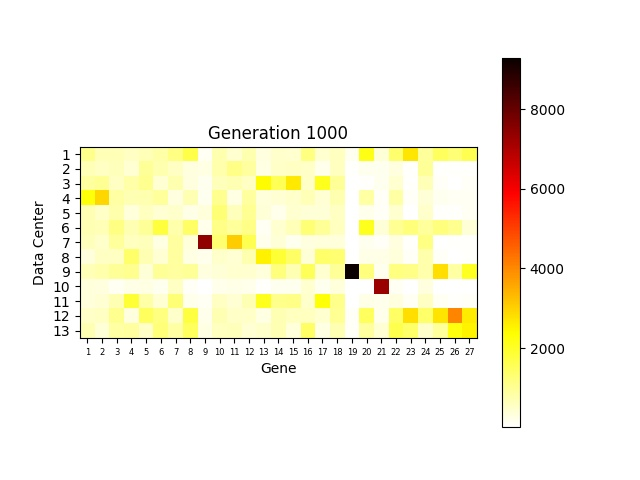
\includegraphics[width=5cm]{Figures/Generation 1000.jpg}
\caption{Generation 1000}
\label{fig:g1000}
\end{minipage}
\begin{minipage}[t]{0.3\linewidth}
\centering
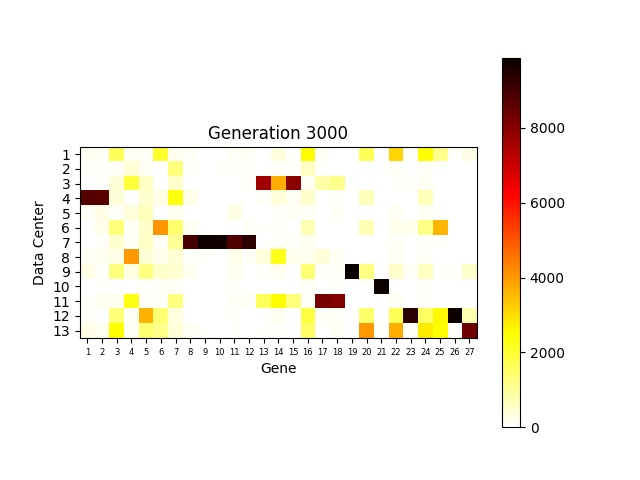
\includegraphics[width=5cm]{Figures/Generation 3000.jpg}
\caption{Generation 3000}
\label{fig:g3000}
\end{minipage}
\end{figure}

\subsection{Small Data Analysis}
After that, we randomly generate some small datasets to further analyze our algorithms' performance. We draw the worst JCT and running time charts (refer to Table~\ref{tab:smallJCT} and Table~\ref{tab:smallRunTime}) as below:
\begin{figure}[htbp]
\centering
\begin{minipage}[t]{0.49\textwidth}
\centering
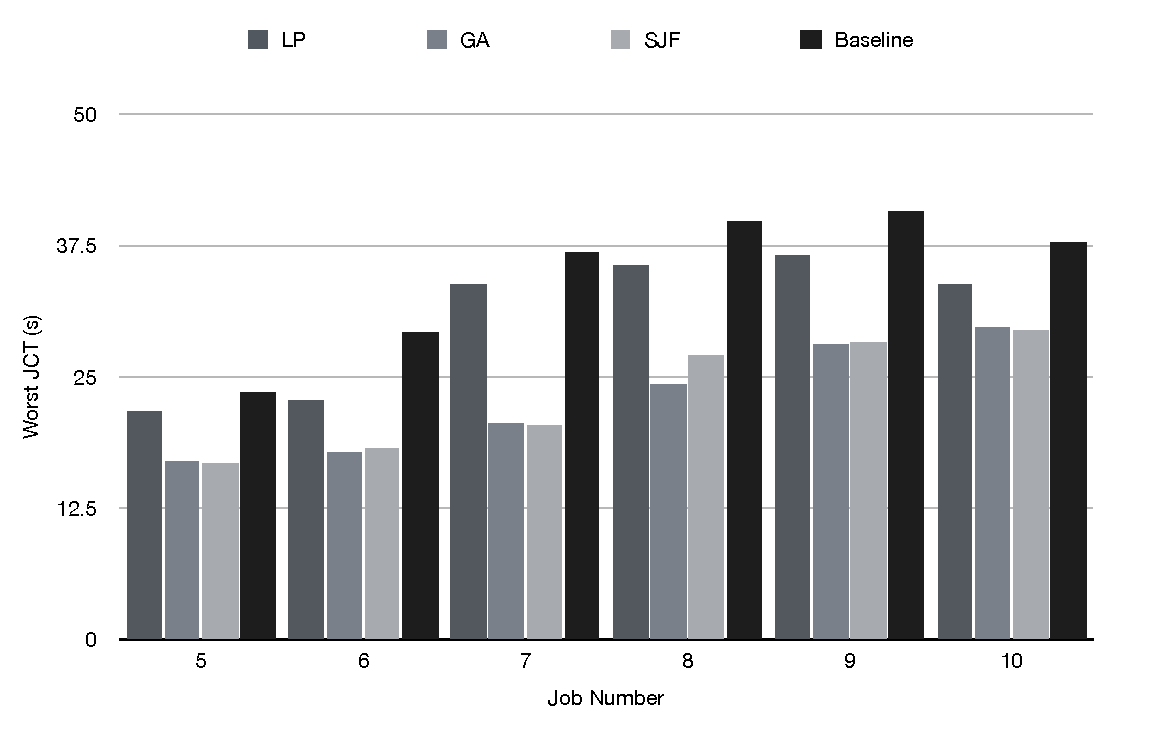
\includegraphics[width=8cm]{Figures/smallJCT.pdf}
\caption{Worst Job Complete Time}
\label{fig:smallJCT}
\end{minipage}
\begin{minipage}[t]{0.49\textwidth}
\centering
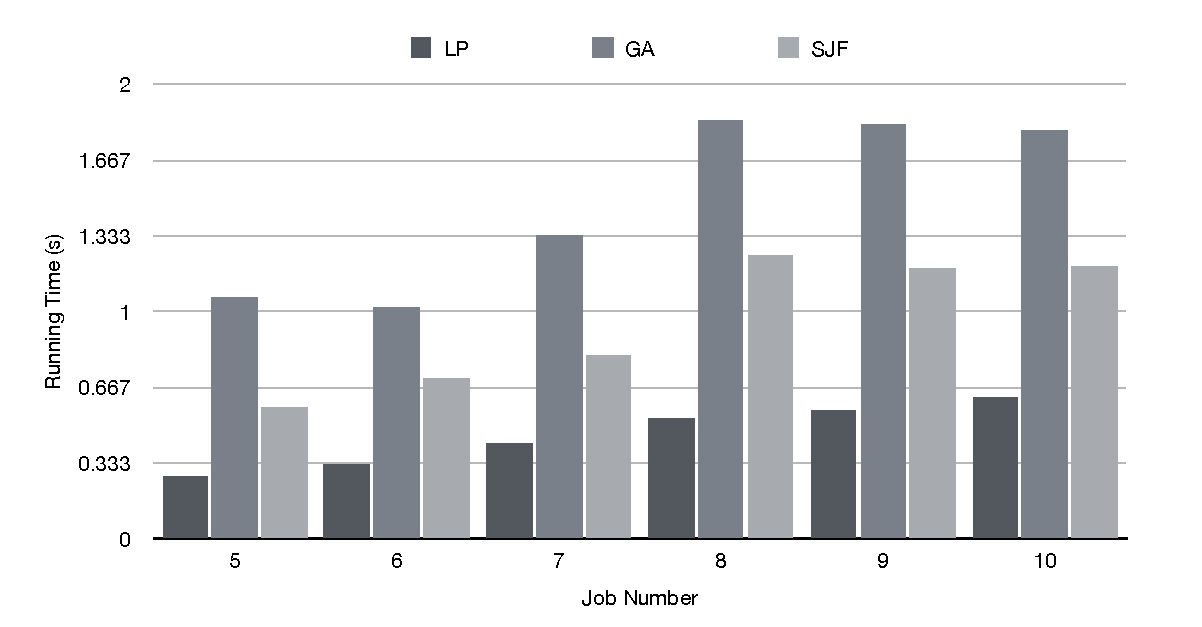
\includegraphics[width=8cm]{Figures/smallRunningTime.pdf}
\caption{Algorithm Running Time}
\label{fig:smallRunning}
\end{minipage}
\end{figure}

From Fig.~\ref{fig:smallJCT}, we could find that all our algorithms always give out results better than the baseline. LP will give a relatively worse job complete time but satisfying strict max-min fairness. Generally, the two random algorithms: GA and SJF Algorithm, will give out close and better results.

From Fig.~\ref{fig:smallRunning}, we could find the same result as what we've discovered on toy data: LP runs fastest, SJF next, and GA relatively slower. 

\subsection{Sensitivity Analysis}
It's an interesting and meaningful job to test our algorithms' sensitivity. Here, we choose the LP algorithm which has two main variables (job threshold and time threshold) to conduct our experiments. The results (refer to Table~\ref{tab:jobSens} and Table~\ref{tab:timeSens}) are shown in the following line charts:
\begin{figure}[htbp]
\centering
\begin{minipage}[t]{0.49\textwidth}
\centering
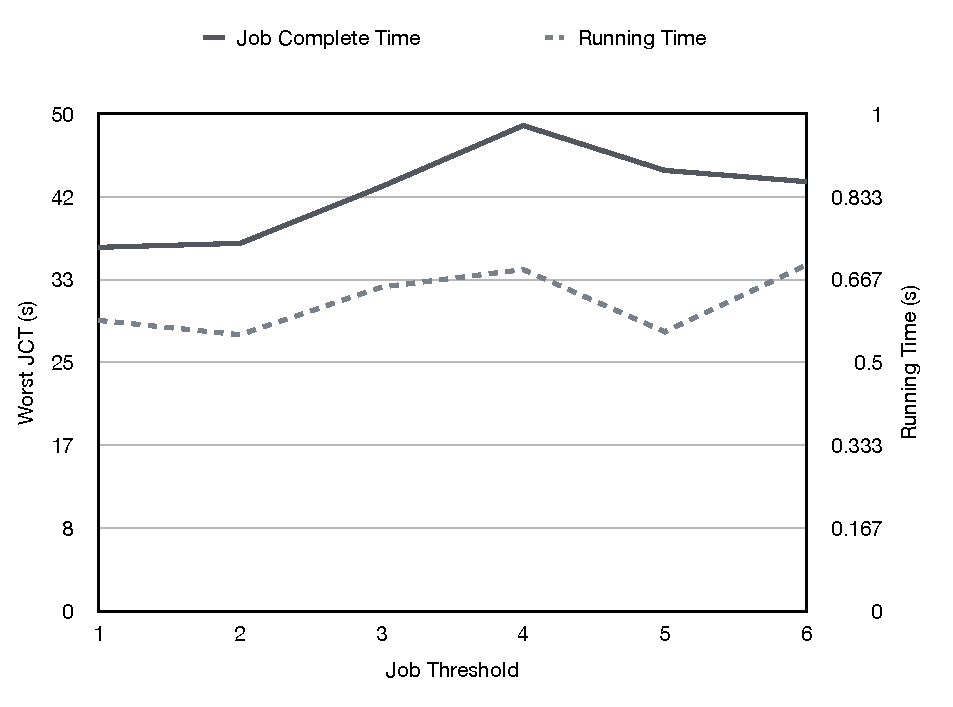
\includegraphics[width=8cm]{Figures/jobThreshold.pdf}
\caption{Job Threshold Analysis}
\label{fig:jobThreshold}
\end{minipage}
\begin{minipage}[t]{0.49\textwidth}
\centering
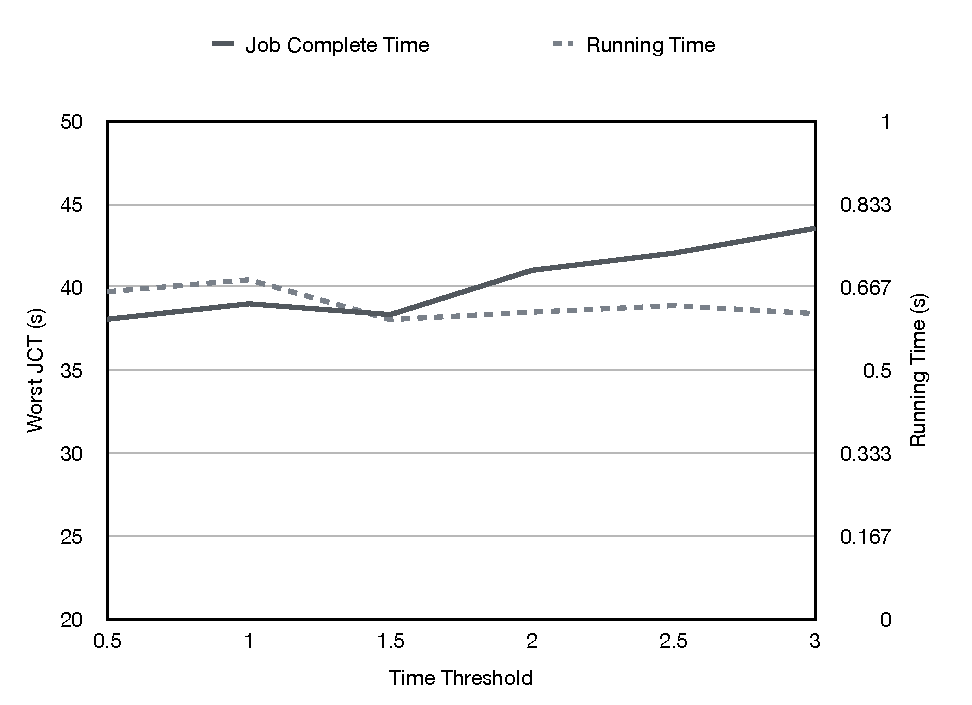
\includegraphics[width=8cm]{Figures/timeThreshold.pdf}
\caption{Time Threshold Analysis}
\label{fig:timeThreshold}
\end{minipage}
\end{figure}

Before discussion, it's necessary for us to have an overview of results' changing regularity. The answer may seem weird, but there doesn't exist tight bound between results and variables. As job threshold growing bigger, the scheduling algorithm will be triggered less. However, since we will have more empty slots during each iteration, the total running time could still be higher. Similarly, though a higher job threshold may put some tasks waiting for more time, they may have a better place to be assigned after waiting, so the worst job complete time may still be reduced. It's exactly the same for time threshold.

So now let's look back on Fig.~\ref{fig:jobThreshold} and Fig.~\ref{fig:timeThreshold}, we could first find that the worst job complete time and program running time have almost the same trend under the changing variables. For job threshold, they may increase then descend. And for time threshold, almost in a stable state, consistent with our expectation.

Job threshold seems to have a bigger influence on the algorithm than the time threshold. For it may have a 30\% fluctuation while the time threshold only 16\%. And after all, the LP algorithm could give out relatively stable results as we could see from the charts.

\section{Test Efficiency on Larger Data}
Finally, we test our algorithms on larger data-sets (Randomly generated, which have 50, 150, 200, 250 jobs to be scheduled).  Based on the results, we draw the worst job complete time chart (refer to Table~\ref{tab:largeJCT}) as following:
\begin{figure}[htbp]
    \centering
    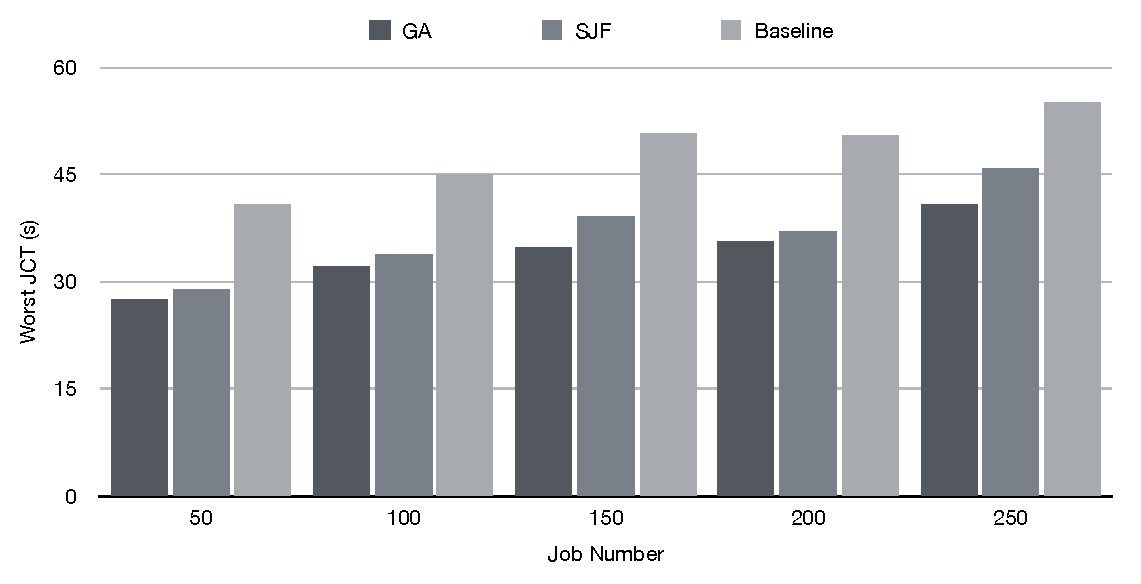
\includegraphics[width=0.8\textwidth]{Figures/largeJCT.pdf}
    \caption{Scheduler Structure}
    \label{fig:largeJCT}
\end{figure}

From Fig.~\ref{fig:largeJCT} we could see that our algorithms could run successfully on big data-sets, always achieving better solutions than the baseline. And a step further, we could find out that the Genetic Algorithm tends to give better task assignment than SJF Algorithm on large data-sets.

\begin{table}[htbp]
    \centering
    \caption{Comparison Of GA Algorithm}
    \begin{tabular}{|c|c|c|c|c|}
    \hline
        {\bf Scale} &JCT1 (s) &Running Time1 (s) &JCT2 (s) &Running Time2 (s) \\ \hline
        50 &28.24 &1.45 &27.26 &21.75 \\ \hline
        100 &33.15 &3.19 &32.82 &22.33 \\ \hline
        150 &35.68 &4.93 &35.12 &24.65 \\ \hline
        200 &36.78 &6.48 &36.61 &25.92 \\ \hline
        250 &40.64 &7.85 &40.28 &27.48 \\ \hline
    \end{tabular}
    \label{tab:GACmp}
\end{table}

Different from the results on small data-sets, the two random algorithm need to run approximately 20 seconds to get a seemly-optimal solution. However, at most time their outputs at the beginning are already great enough to be a reasonable solution as shown in Table~\ref{tab:GACmp}. Further considering the limited computation capability of our laptops, the two algorithms could be more useful when we have enough computation resources.
 
\section{Conclusion}
To summarize all that we've discussed above, we draw the following conclusions:
\begin{itemize}
    \item We define symbols and transform the {\bf max-min fairness} into lexicographical order. Furthermore, we formalize the problem with notations and set clear targets for our algorithms.
    
    \item We conduct detailed proof to claim that the multi-job scheduling problem is in NP-Complete.
    
    \item We design three effective algorithms: Genetic Algorithm (average in polynomial time), Shortest Job First (SJF) Algorithm (average in polynomial time) and Linear Programming (average in polynomial time) to solve the problem.
    
    \item We conduct experiments on the toy data using the three algorithms above, find the shortest worst job complete time to be 17.65s while the average computation time is 7.54s.
    
    \item We test our algorithms' efficiency on randomly-generated small and big data-sets and find out that: all three algorithms give out better scheduling than the baseline, LP runs relatively faster while GA and SJF could often yield assignments with shorter complete time.  
    
    \item We also do sensitivity analysis and many other meaningful visualization to further prove our algorithms' efficiency.
\end{itemize}

\section*{Acknowledgements}
First of all, we would like to praise the tacit cooperation of our team. Although every member in our team is only responsible for his algorithm, we all work together to accomplish all tasks during the final integration of the draft.

Secondly, we would like to thank the teaching assistants for this course. We encountered several problems when completing with the project, the two teaching assistants answered our questions one by one with patience.

Thanks to Prof. Gao and Mr. Li for bringing us project problems together. In the process of completing this task, our group is like playing a mathematical modeling contest to catch a glimpse of the charm of the algorithm from the novel dimension of problem solving. In the process of solving this problem, we fully feel the importance of team cooperation, and the great improvement of excellent algorithm in time cost.

Finally, we cannot emphasize more on thanking Mrs. Xiaofeng Gao and Mr. Lei Wang, who have made great efforts in the course of algorithm. It is Mrs. Gao who taught us linear programming algorithm, CPLEX solver and data visualization method. In the process of writing this paper, the use of solvers, data visualization methods, greedy algorithm and other contents taught by the teachers are all in use. It can be said that the course of algorithm has large capacity and many contents, which not only enriches our empty spare time, but also irrigates our brain with rigorous computer thinking.  

%
% ---- Bibliography ----
%
% BibTeX users should specify bibliography style 'splncs04'.
% References will then be sorted and formatted in the correct style.
%
% \bibliographystyle{splncs04}
% \bibliography{mybibliography}
%
\begin{thebibliography}{8}

\bibitem{ref_6}
Vijay V Vazirani. Approximation algorithms. Springer Science \& Business Media, 2013.

\bibitem{ref_7}
Eva Hopper and Brian CH Turton. A review of the application of meta-heuristic algorithms to 2d strip packing problems. Artificial Intelligence Review, 16(4):257–300, 2001.

\bibitem{ref_8}
Silvano Martello, David Pisinger, and Daniele Vigo. The three-dimensional bin packing problem. Operations research, 48(2):256–267, 2000.

\bibitem{ref_9}
Zhigang Hua, Qi Feng, Gan Liu, Shuang Yang. Learning to Schedule DAG Tasks. arXiv:2103.03412, Mar 2021.

\bibitem{ref_10}
Travelling Salesman Problem(TSP) - Wikipedia,
\url{https://en.wikipedia.org/wiki/Travelling\_salesman\_problem}.

\bibitem{ref_11}
Li Chen, Shuhao Liu, Baochun Li, and Bo Li, Scheduling Jobs across Geo-Distributed Datacenters with MaxMin Fairness, IEEE Transactions on Network Science and Engineering (TNSE), 6(3):488-500, 2019.

\bibitem{ref_12}
Dritan Nace and Michal Pioro, Max-Min Fairness and its Applications to Routing and Load-Balancing in Communication Networks: A Tutorial, IEEE Communications Surveys and Tutorials, 10(1-4): 5-17, 2008.

\bibitem{ref_13}
Simplex Algorithm - Wikipedia,
\url{https://en.wikipedia.org/wiki/Simplex\_algorithm}.

\end{thebibliography}

\section*{Appendix}
We list experiments data that hasn't been shown in the text in this section.

\begin{table}[htbp]
    \centering
    \begin{minipage}[t]{0.49\textwidth}
    \centering
    \caption{Small Data Running Time Comparison}
    \begin{tabular}[width=8cm]{|c|c|c|c|}
    \hline
    Job Number  & LP (s) & GA (s) & SJF (s)  \\ \hline
    5  & 0.278 & 1.066 & 0.573 \\ \hline
    6 & 0.326 & 1.019 & 0.701 \\ \hline
    7 & 0.419 & 1.341 & 0.804 \\ \hline
    8 & 0.535 & 1.840 & 1.250 \\ \hline
    9 & 0.565 & 1.826 & 1.187 \\ \hline
    10 & 0.627 & 1.795 & 1.201 \\ \hline
    \end{tabular}
    \label{tab:smallRunTime}
    \end{minipage}
    \begin{minipage}[t]{0.49\textwidth}
    \centering
    \caption{Small Data Worst JCT Comparison}
    \begin{tabular}[width=8cm]{|c|c|c|c|c|}
    \hline
    Job Number  & LP (s) & GA (s) & SJF (s) & Baseline (s) \\ \hline
    5  & 21.803 & 16.893 & 16.755 & 23.400 \\ \hline
    6 & 22.625 & 17.655 & 18.227 & 29.280\\ \hline
    7 & 33.824 & 20.529 & 20.278 & 36.740 \\ \hline
    8 & 35.494 & 24.291 & 27.001 & 39.830 \\ \hline
    9 & 36.586 & 28.102 & 28.207 & 40.732 \\ \hline
    10 & 33.787 & 29.663 & 29.393 & 37.800 \\ \hline
    \end{tabular}
    \label{tab:smallJCT}
    \end{minipage}
\end{table}

\begin{table}[htbp]
    \centering
    \centering
    \caption{Large Data Worst JCT Comparison}
    \begin{tabular}[width=8cm]{|c|c|c|c|}
    \hline
    Job Number  & GA (s) & SJF (s) & Baseline (s) \\ \hline
    50  & 27.273 & 28.810 & 40.920 \\ \hline
    100 & 32.170 & 33.740 & 44.780 \\ \hline
    150 & 34.573 & 38.967 & 50.790  \\ \hline
    200 & 35.576 & 36.940 & 50.410 \\ \hline
    250 & 40.690 & 45.806 & 55.190 \\ \hline
    \end{tabular}
    \label{tab:largeJCT}
\end{table}

\begin{table}[htbp]
    \centering
    \begin{minipage}[t]{0.49\textwidth}
    \centering
    \caption{Job Threshold Analysis}
    \begin{tabular}{|c|c|c|}
    \hline
    Job Threshold  & JCT (s) & Running time (s) \\ \hline
    1 & 36.586 & 0.585 \\ \hline
    2 & 36.988 & 0.556  \\ \hline
    3 & 42.690 & 0.652   \\ \hline
    4 & 48.820 & 0.687  \\ \hline
    5 & 44.310 & 0.562  \\ \hline
    6 & 43.180 & 0.696  \\ \hline
    \end{tabular}
    \label{tab:jobSens}
    \end{minipage}
    \begin{minipage}[t]{0.49\textwidth}
    \centering
    \caption{Time Threshold Analysis}
    \begin{tabular}{|c|c|c|}
    \hline
    Time Threshold  & JCT (s) & Running time (s) \\ \hline
    0.5 & 38.080 & 0.658 \\ \hline
    1.0 & 39.010 & 0.682  \\ \hline
    1.5 & 38.360 & 0.602   \\ \hline
    2.0 & 41.030 & 0.617  \\ \hline
    2.5 & 42.060 & 0.630  \\ \hline
    3.0 & 43.560 & 0.614  \\ \hline
    \end{tabular}
    \label{tab:timeSens}
    \end{minipage}
\end{table}

\end{document}
